%%%%%%%%%%%%%%%%%%%%%%%%%%%%%%%%%%%%%%%%%%%%%%%%%%%%%%%%%%%%%%%%%%%%%%%%%%%%%%%%
%%                           ONDER DE LOEP ARTIKEL                            %%
%%%%%%%%%%%%%%%%%%%%%%%%%%%%%%%%%%%%%%%%%%%%%%%%%%%%%%%%%%%%%%%%%%%%%%%%%%%%%%%%

	
\artikelfoto{Determinanten}{}{Michel Roelens \\ Mathias Stichelbaut \\ Luc Van den Broeck}{img/bannerdeterminant.jpg}

\startcontents[inhoudloep]	% om inhoud voor het loep artikel te beginnen

\begin{multicols}{2}
	
	\inhoudstafelloep			% om inhoudstafel voor het loep artikel te tonen
	
	%% Gebruik \section{titel} en \subsection{titel} om genummerde tussentitels te maken
\section{Inleiding}

Na lange tijd zijn de determinanten terug van weggeweest. Ze zijn niet meer louter een keuzeonderwerp voor de trouwe liefhebbers maar ze staan nu als volwaardig item in de specifieke eindtermen (bij de gevorderde wiskunde) en dus ook in de verschillende recent goedgekeurde leerplannen. 

In het \emph{leerplan Wiskunde B+S''} van het KOV staat bij LPD 36 dat de determinant van een vierkante matrix berekend moet kunnen worden. De doelstelling laat in het midden of dit manueel of met software gebeurt en ook voor welk formaat van matrices dit moet gebeuren. De wenken geven aan dat het verband `kan' gelegd worden met de oplosbaarheid van stelsels en met de inverteerbaarheid van vierkante matrices. Deze twee invalshoeken werken wij uit in respectievelijk paragraaf 2 en paragraaf 3. We belichten dus twee sporen die leiden naar het determinantbegrip. 

Bij LPD 6 lezen we bij de wenken dat de cartesiaanse vergelijking van een vlak in determinantvorm kan geschreven worden. In paragraaf 2 leiden we LPD6 in met de determinantvergelijking van een rechte. We gaan dan verder met de vergelijking van een vlak en met de vergelijking van een parabool door drie gegeven punten.

Het \emph{leerplan van het GO!} loopt vrij gelijkaardig. Bij de doorstroomrichting wetenschappen-wiskunde worden ook de eigenschappen van determinanten belicht. Deze eigenschappen nemen we alleen op in het tweede spoor van deze loep dat iets diepgaander is dan het eerste, zie paragraaf 3.

Het \emph{Wiskundeplan}, eveneens goedgekeurd door de onderwijsinspectie voor de richtingen met zes uur wiskunde in de derde graad, gaat ook iets dieper in op de eigenschappen en op de meetkundige toepassingen. Het Wiskundeplan neemt bovendien de regel van Cramer op. Hoe we deze uitgebreidere leerlijn strak uit kunnen werken, verneem je in paragraaf 3.

Paragraaf 4 is een uitstapje voor leerlingen en leerkrachten die de determinant tastbaar willen maken via oppervlakten van parallellogrammen en inhouden van parallellepipeda. Uit deze meetkundige interpretatie volgen enkele mooie eigenschappen. Als je de determinant meetkundig interpreteert, is het niet meer mogelijk deze eigenschappen niet te begrijpen of ze te vergeten.

Deze loep is geen pleidooi voor of tegen determinanten. Wel willen we inspelen op de nieuwe leerplansituatie waarin de determinanten tot de vaste leerstof behoren in de richtingen met component wiskunde. In de jaren '90 maakten we een omgekeerde leerplanwijziging mee. Determinanten verdwenen uit het leerplan voor richtingen met zes uur wiskunde. Sommige leerkrachten vroegen zich toen bijvoorbeeld af hoe je de vergelijking van een vlak in de ruimte kunt opstellen zonder determinanten. We legden toen uit dat dit perfect gaat met de methode van Gauss-Jordan. Nu zijn we een generatie verder en kunnen we uitleggen hoe je de vergelijking van een vlak ook met determinanten kunt aanbrengen. 

Het voordeel van het oplossen van stelsels met determinanten in plaats van met de methode van Gauss-Jordan zit niet in een reductie van het aantal uit te voeren bewerkingen. Nee, het mooie eraan is dat je een formule kunt geven die de oplossing van een stelsel geeft in functie van de coëfficiënten van de vergelijkingen, op dezelfde manier als je een formule kunt geven voor bijvoorbeeld de oplossingen van een tweedegraadsvergelijking. Adepten van deze structuur zullen de komende jaren weer volop aan hun trekken kunnen komen.

\end{multicols}
 \afbeelding[0.7\textwidth]{./tekeningenKurt/determinatie.jpg}{}{}
\begin{multicols}{2}
\section{Het eerste spoor naar de determinanten}

Het eerste spoor naar de determinanten is een spoor dat snel is maar iets minder diepgang heeft. Als je een leerlingengroep een stevigere uitdaging aankan, hoef je de determinanten niet op deze manier te introduceren. Je kiest dan beter voor het tweede spoor.

We starten hier met een werktekst waarvoor geen basiskennis vereist is tenzij die van stelsels met twee vergelijkingen en twee onbekenden. Die hebben de leerlingen in de tweede graad gekregen bij de berekening van de snijpunten van twee rechten. De overgang naar vergelijkingen met algemene coëfficiënten is hier nieuw. 

\end{multicols}
\begin{lesactiviteit}{Homogene $2 \times 2$-stelsels}

Het stelsel
\[ \left\{ \begin{aligned} 
        2x+3y & = 0 \\
        4x+7y &= 0
\end{aligned} \right. \]
is een \emph{homogeen} stelsel met twee vergelijkingen en twee onbekenden. We noemen dit stelsel van eerste graadsvergelijkingen \emph{homogeen} omdat de constante termen gelijk zijn aan 0. Er komen veelvouden van $x^1$ en $y^1$ voor. De exponenten van $x$ en $y$ zijn \emph{homogeen}. 

De coëfficiënten bij de onbekenden $x$ en $y$ kunnen we samenvatten in een getallentabel of een \emph{matrix}. Deze matrix noemen we de \emph{coëfficiëntenmatrix} van het homogene stelsel:
\[ \left( \begin{matrix}
    2 & 3 \\
    4 & 7
\end{matrix} \right). \]

\begin{vraagenantwoord}
    \vraag{Is dit stelsel strijdig? Formuleer je antwoord zonder schriftelijke berekeningen te maken.}
    \antwoord{Neen, het stelsel is niet strijdig. Je kunt meteen een oplossing aflezen nl. $(0,0)$. Dit is niet verwonderlijk: alle homogene stelsels hebben dezelfde vanzelfsprekende nuloplossing. We noemen ze de \emph{triviale} oplossing.}
		
    \vraag{Zijn er nog andere oplossing?}
    \antwoord{Neen, de triviale oplossing is de enige. Dit kun je op verschillende manieren narekenen, bijvoorbeeld met de combinatiemethode. Als je van de tweede vergelijking twee keer de eerste aftrekt, stel je vast dat $y$ gelijk aan 0 is. Hieruit volgt dan meteen dat ook $x$ gelijk is aan 0. Maar je de leerlingen ook vragen om een redenering met de substitutiemethode te maken.}
\end{vraagenantwoord}

Een stelsels met precies één oplossing, noemen we een \emph{bepaald stelsel}. Maar niet alle homogene $2 \times 2$-stelsels zijn bepaald. Neem bijvoorbeeld het homogene stelsel met coëfficiëntenmatrix $\pmM{14 & 21 \\ 10 & 15}$.

\begin{vraagenantwoord}[resume]
    \vraag{Toon aan dat het homogene stelsel met deze coëfficiëntenmatrix oneindig veel oplossingen heeft.}
    \antwoord{De handigste methode is hier om de eerste vergelijking te delen door 7 en de tweede door 5. We krijgen dan twee identieke vergelijkingen: 2x+3y=0. Een van deze twee vergelijkingen mogen we weglaten omdat ze geen extra informatie geeft. De meest voor de hand liggende oplossing voor de overblijvende vergelijking is $(3,-2)$. Maar ook $(33,-22)$ is een correcte oplossing. Concreet: alle veelvouden van $(3,-2)$ zijn oplossingen. Het stelsel met coëfficiëntenmatrix $\pmM{14 & 21 \\ 10 & 15}$ is dus niet bepaald.}
\end{vraagenantwoord}

Een stelsel met een oneindig aantal oplossingen noemen we een \emph{onbepaald stelsel}. Homogene $2 \times 2$-stelsels kunnen zowel bepaald als onbepaald zijn. Van beide gevallen gaven we een voorbeeld. 

We onderzoeken in deze werktekst verder hoe we vanuit de coëfficiëntenmatrix van een homogeen $2 \times 2$-stelsel kunnen zien of het stelsel bepaald of onbepaald is. 

\begin{vraagenantwoord}[resume]
    \vraag{Wanneer is het homogene $2 \times 2$-stelsel met coëfficiëntenmatrix $\pmM{a & b \\ c & d}$ bepaald?}
    \antwoord{We schetsen hier een antwoord via de substitutiemethode. \\ Als $a \neq 0$ dan leiden we uit de vergelijking $ax+by=0$ een uitdrukking voor $x$ af. We vervangen de onbekende $x$ in de vergelijking $cx+dy=0$ door $-\frac{by}{a}$. Na de vermenigvuldiging van beide leden met de noemer $a$ vinden we de vergelijking $(ad-bc)y=0$. Deze vergelijking geeft uitsluitsel over het aantal oplossingen. Als $ad-bc\neq 0$ dan heeft deze vergelijking slechts één oplossing. Als $ad-bc = 0$ dan heeft deze vergelijking oneindig veel oplossingen. Alle reële getallen kunnen immers ingevuld worden in de vergelijking $0y=0$.\\
    Merk op dat deze redenering alleen opgaat als $a\neq 0$. Als $a=0$ en $c\neq 0$ dan kunnen we dezelfde voorwaarde vinden door de waarde van $x$ te berekenen uit de tweede vergelijking ($x=-\frac{dy}{c}$) en die in de eerste vergelijking in te vullen.\\ Het geval waarin $a=c=0$ komt niet voor. We hebben in dit geval immers geen homogeen $2 \times 2$-stelsel. Alleen de onbekende $y$ komt dan in het stelsel voor.}
\end{vraagenantwoord} 

Elke $2 \times 2$-matrix kan beschouwd worden als de coëfficiëntenmatrix van een homogeen $2 \times 2$-stelsel.  Voor de matrix $\pmM{a & b \\ c & d}$ is het getal $ad-bc$ cruciaal om te weten of het om een bepaald of om een onbepaald stelsel gaat. De determinant van de coëfficiëntenmatrix is een getal dat door zijn al of niet nul-zijn bepaalt in welke situatie we ons bevinden. Als de determinant nul is, dan is het stelsel onbepaald. Als de determinant van nul verschilt, dan is het stelsel bepaald. \emph{Determineren} betekent trouwens \emph{bepalen}. Een \emph{determinant} is een \emph{getal dat iets bepaalt}. 

We noteren de determinant van een matrix door de letters \emph{det} voor de matrix te zetten of door de vervanging van de ronde haken van de matrix door verticale lijnen. Deze twee notaties worden in de literatuur door elkaar gebruikt.\\

\begin{kader}{Definitie}{Determinant van een $2 \times 2$-matrix}
\[\det \left( \begin{aligned} a \quad & b \\ c \quad & d  \end{aligned}  \right) = \left| \begin{aligned} a \quad & b \\ c \quad & d  \end{aligned}  \right| = ad-bc\]   
\end{kader}

\begin{vraagenantwoord}[resume]
    \vraag{Voor welke waarden van $m$ is het volgende stelsel onbepaald? Beantwoord deze vraag via een determinantberekening.
    \[ \left\{ \begin{aligned} 
        & mx  -  4y & = 0 \\
        & 3x  +  (m-7)y &= 0
        \end{aligned} \right. \]}
    \antwoord{De voorwaarde voor de onbepaaldheid is $\dmM{m & -4 \\ 3 & m-7}=0$. Via de determinantformule leidt dit tot $m(m-7)-(-4)3=0$ of tot $m^2-7m+12=0$. Door deze vierkantsvergelijking op te lossen, bijvoorbeeld met de som- en productformule, kunnen we besluiten dat het stelsel onbepaald is voor $m=3$ en voor $m=4$. In alle andere gevallen heeft het stelsel slechts één oplossing, nl. $(0,0)$.}
\end{vraagenantwoord}
\end{lesactiviteit}

\begin{multicols}{2}

\subsection{De determinant van een $3 \times 3$-matrix}

Bij homogene $3 \times 3$-stelsels is het niet zo eenvoudig om deze berekeningen manueel over te doen. We moeten hier immers rekening houden met 9 coëfficiënten. De berekeningen worden overduidelijk een hard labeur. We kunnen ons echter laten bijstaan door GeoGebra. In het CAS-scherm wordt rekenen met letters een makkie. Toegegeven, wat betreft noemers die mogelijk gelijk kunnen zijn aan nul, gaat GeoGebra er met vuile voeten door. Maar in deze fase van het onderzoek schuiven we dit probleem even aan de kant.  

Door drie substituties uit te voeren, leiden we uit het gegeven stelsel 
\[ \left\{ \begin{aligned} 
        a_1 x+b_1 y+c_1 z & = 0 \qquad \qquad (1)\\
        a_2 x+b_2 y+c_2 z & = 0 \qquad \qquad (2)\\
        a_3 x+b_3 y+c_3 z & = 0 \qquad \qquad (3)
\end{aligned} \right. \]
één vergelijking af met één enkele onbekende. We leggen in stapjes uit hoe we dit doen.

Eerst halen we de onbekende $x$ uit vergelijking (1) en substitueren we de gevonden uitdrukking in (2) en in (3), zie \autoref{vervang1}. Hiervoor zijn twee GeoGebra-commando's nodig: Oplossen en Vervangen. Zo is het stelsel gereduceerd van formaat $3 \times 3$ naar formaat $2 \times 2$. De nieuwe vergelijkingen worden hier benoemd met de letters $s$ en $t$.

\end{multicols}

\afbeelding [15cm]{img/vervangen1.jpg}{De eerste substitutie}{vervang1}

\begin{multicols}{2}

Daarna halen we de onbekende $y$ uit vergelijking $s$ en vervangen we deze onbekende in vergelijking $t$. Dit zie je in \autoref{vervang2}.

Het resultaat van deze substituties is één vergelijking in één onbekende. Deze vergelijking wordt benoemd met de letter $v$. Het linkerlid kan in factoren ontbonden worden door de onbekende $z$ af te zonderen. Eventueel kan ook de noemer nog weggewerkt (of weggedacht) worden door beide leden met $a_1 b_2-a_2 b_1$ te vermenigvuldigen. Daarna zou het duidelijk moeten zijn wanneer de resulterende  vergelijking (en dus ook het gegeven stelsel) onbepaald is.

\end{multicols}

\afbeelding [15cm]{img/vervangen2.jpg}{De tweede en derde substitutie}{vervang2}

\begin{multicols}{2}

Analoog aan de afleiding voor $2 \times 2$-stelsels gebeurt dit wanneer de coëfficiënt van $z$ gelijk is aan 0. Deze coëfficiënt bestaat uit drie termen met een plusteken en drie termen met een minteken. 

In het geval dat de leerlingen voortdurend over een computer kunnen beschikken, heeft het weinig zin om deze formule uit het hoofd te leren. Ze kunnen deze determinant ook met een korte instructie opvragen in GeoGebra. Even uittesten of dit werkt, is zeker de moeite, zie \autoref{vervang3}. Vanaf nu mag de determinantberekening van een $3\times3$-matrix (de regel van Sarrus) als een blackbox gehanteerd worden. De leerlingen hoeven zich niet voortdurend meer te realiseren dat er een aantal substituties achter het oplossen van een stelsel zitten. 


\end{multicols}

\afbeelding [15cm]{img/vervangen3.jpg}{De determinantberekening in één stap}{vervang3}

\begin{multicols}{2}

Dat het rekenwerk doorgeschoven wordt naar GeoGebra betekent niet dat er niet meer geredeneerd hoeft te worden. In tegendeel zelfs. Hoe meer het algebraïsche rekenwerk wordt doorgeschoven, hoe kritischer de leerlingen moeten staan tegenover het resultaat. 

De vraag waarom de determinant van een matrix met twee gelijke rijen of met twee gelijke kolommen altijd gelijk is aan 0 is bijvoorbeeld bijzonder interessant. Om deze vraag te beantwoorden, kunnen de leerlingen steunen op de de rang van de rijherleide matrix, als dit onderwerp al behandeld is in de les. Maar ze kan ook beredeneerd worden zonder enige specifieke bagage.

We bekijken als voorbeeld een $3 \times 3$-matrix met twee gelijke rijen:

\[ \left( \begin{matrix}
    a & b & c \\
    d & e & f \\
    d & e & f
\end{matrix} \right). \]

die aanleiding geeft tot het homogene stelsel:

\[\left\{ 
\begin{aligned} ax+by+cz&=0 \\ dx+ey+fz&=0 \\  dx+ey+fz&=0 \end{aligned}  
\right.\]

waarvan de laatste vergelijking geen bijkomende informatie geeft. De derde vergelijking mag dus weggelaten worden. Als we de derde onbekende naar het linkerlid brengen, hebben we opnieuw een vierkant stelsel.

\[\left\{ 
\begin{aligned} ax+by&=-cz \\ dx+ey&=-fz \end{aligned}  
\right..\]

Als $(a,b)$ een veelvoud is van $(c,d)$ dan kiezen we $z$ gelijk aan nul. Het stelsels heeft dan oneindig veel oplossingen want het is homogeen en de determinant is gelijk aan nul. Als $(a,b)$ geen veelvoud is van $(c,d)$ dan heeft het stelsel één enkele oplossing voor elke waarde van $z$ die we vrij kunnen kiezen. Ook in dit geval zijn er dus oneindig veel oplossingen te vinden. 

Hiermee is aangetoond dat een $3 \times 3$-stelsel met twee gelijke vergelijkingen altijd een oneindig aantal oplossingen heeft en dat de determinant van een $3 \times 3$-matrix dus gelijk aan nul is.

We laten het aan de lezer over om een bewijs zonder achtergrondkennis te zoeken voor de (vast)stelling dat de determinant van een $3 \times 3$-matrix met twee gelijke kolommen gelijk aan nul is. 


\subsection{De determinantvergelijking van een rechte}

In de tweede graad maakten de leerlingen kennis met de cartesiaanse vergelijking van een rechte bepaald door twee punten. Deze vergelijkingen werden in de vorm $y=ax+b$ geschreven en in de vorm $px+qy+r=0$. De werktekst hieronder begint met een korte herhaling.

\end{multicols}
\begin{lesactiviteit}{De vergelijking van een rechte via determinanten}
	
\begin{vraagenantwoord}
    
    \vraag{Hieronder zie je een rechte die door twee gegeven punten gaat. Vorig jaar heb je twee verschillende vergelijkingen voor zulke rechten opgesteld. Eentje was van de vorm $px+qy+r=0$, de tweede was van de vorm $y=ax+b$. Stel deze twee vergelijkingen op van de onderstaande rechte. }
    \antwoord{Met de kennis van de cartesiaanse vergelijking van de rechte door twee gegeven punten vinden we de vergelijking $y=-\frac{1}{2}x+\frac{7}{2}$. Door een factor en daarna een term over te brengen zetten we deze vergelijking om in $x+2y-7=0$.}
\end{vraagenantwoord}
\ \\
\begin{center}
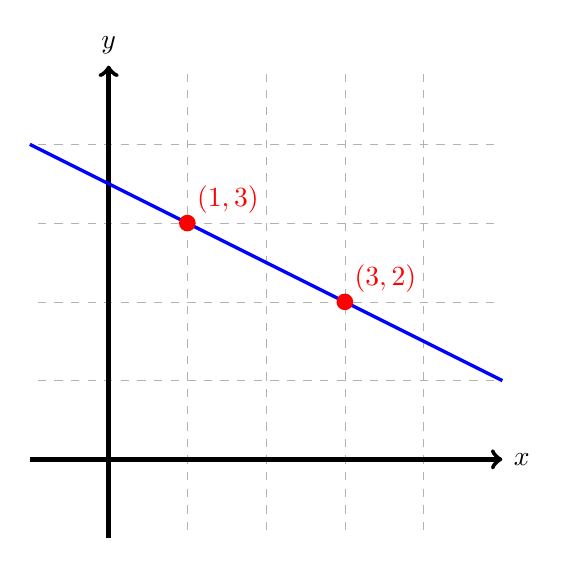
\begin{tikzpicture}
\draw[help lines, color=gray!60, dashed] (-0.9,-0.9) grid (4.9,4.9);
\draw[->,ultra thick] (-1,0)--(5,0) node[right]{$x$};
\draw[->,ultra thick] (0,-1)--(0,5) node[above]{$y$};
\draw[very thick, blue] (-1,4)--(5,1);
\coordinate (A) at (1,3);
\fill[red] (A) circle (3pt);
\node [above right,  red] at (A) {$(1,3)$};
\coordinate (B) at (3,2);
\fill[red] (B) circle (3pt);
\node [above right, red] at (B) {$(3,2)$};
\end{tikzpicture} 
\end{center}
\ \\
\begin{vraagenantwoord}[resume]
    \vraag{Zijn er bij de eerste vorm nog andere waarden van $p$,$q$ en $r$ mogelijk? En zijn er bij de tweede vorm nog andere waarden voor $a$ en $b$ mogelijk?}
    \antwoord{Er zijn geen andere waarden mogelijk voor $a$ en $b$ want $a$ is de richtingscoëfficiënt van de rechte en $b$ is het snijpunt met de $y$-as. Maar er zijn wel andere waarden voor $p$, $q$ en $r$ mogelijk, bijvoorbeeld $11$, $22$ en $-77$. Voor het drietal $(p, q, r)$ leveren alle waarden $(\alpha, 2\alpha, -7\alpha)$  met $\alpha \neq 0$ een vergelijking op van de rechte op de figuur.}
\end{vraagenantwoord}
\ \\

Door dit onbegrensde aantal mogelijkheden voor het drietal $(p, q, r)$ kunnen we de link leggen met de onbepaalde homogene vierkante stelsels. We zoeken in deze werktekst een vergelijking van de rechte door twee gegeven punten: $(x_1,y_1)$ en $(x_2,y_2)$. Hierbij kiezen we voor de vergelijking $px+qy+r=0$. Om deze rechte eenduidig te kunnen omschrijven is het nodig waarden voor $p$, $q$ en $r$ te bepalen.

\begin{center}
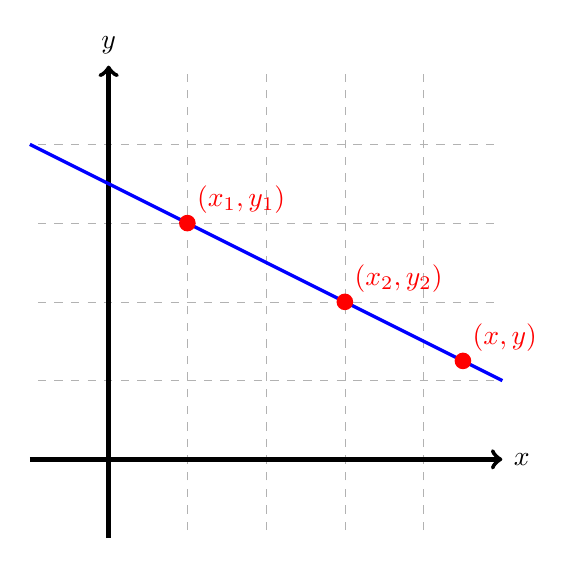
\begin{tikzpicture}
\draw[help lines, color=gray!60, dashed] (-0.9,-0.9) grid (4.9,4.9);
\draw[->,ultra thick] (-1,0)--(5,0) node[right]{$x$};
\draw[->,ultra thick] (0,-1)--(0,5) node[above]{$y$};
\draw[very thick, blue] (-1,4)--(5,1);
\coordinate (A) at (1,3);
\fill[red] (A) circle (3pt);
\node [above right,  red] at (A) {$(x_1,y_1)$};
\coordinate (B) at (3,2);
\fill[red] (B) circle (3pt);
\node [above right, red] at (B) {$(x_2,y_2)$};
\coordinate (C) at (4.5,1.25);
\fill[red] (C) circle (3pt);
\node [above right, red] at (C) {$(x,y)$};
\end{tikzpicture} 
\end{center}

\begin{vraagenantwoord}[resume]
    \vraag{Druk uit dat een willekeurig punt $(x,y)$ op de rechte ligt. Druk daarna uit dat de gegeven punten $(x_1,y_1)$ en $(x_2,y_2)$ op de rechte liggen.}
    \antwoord{Een punt ligt op een gegeven rechte als de coördinaten van dit punt ingevuld kunnen worden in de vergelijking van de rechte (zo dat de gelijkheid klopt). We mathematiseren deze drie voorwaarden als volgt:}
    \[
        \left\{ 
        \begin{aligned}
        p x+q y +r&=0 \\
        p x_1+q y_1 +r&=0 \\
        p x_2+q y_2 +r&=0         
        \end{aligned} 
        \right..
    \]
\end{vraagenantwoord}   

De moeilijkste stap in de redenering is een blikwissel. Je bent gewoon om de letters $x$ en $y$ als onbekenden te zien. Maar nu zijn we op zoek naar de waarden van $p$, $q$ en $r$.

\begin{vraagenantwoord}[resume]
    \vraag{Bekijk dit stelsel met een blikwissel en bepaal de coëfficiëntenmatrix van dit nieuwe stelsel.}
    \antwoord{De blikwissel kun je maken door de onbekenden in kleur te zetten en de coëfficiënten voor de onbekenden te zetten.    
    \[
        \left\{ 
        \begin{aligned}
        x \cdot \textcolor{red}{p}+y \cdot \textcolor{red}{q}+1 \cdot \textcolor{red}{r}&=0 \\
        x_1 \cdot \textcolor{red}{p}+y_1 \cdot \textcolor{red}{q}+1 \cdot\textcolor{red}{r}&=0 \\
        x_2 \cdot \textcolor{red}{p}+y_2 \cdot \textcolor{red}{q}+1 \cdot \textcolor{red}{r}&=0 
        \end{aligned} 
        \right.
    \]
    De coëfficiëntenmatrix wordt nu:
    \[\left( \begin{matrix}
     x & y & 1 \\
    x_1 & y_1 & 1 \\
    x_2 & y_2 & 1
\end{matrix} \right)\]}

    \vraag{Wat weet je van de determinant van deze coëfficiëntenmatrix? Beargumenteer je antwoord.}
    \antwoord{De determinant van de coëfficiëntenmatrix is gelijk aan nul want het bijbehorend homogene stelsel is onbepaald. De onbepaaldheid werd aangetoond in vraag 2.}
\end{vraagenantwoord}

Zo vinden we een nieuwe uitdrukking van de vergelijking van een rechte door twee gegeven punten.\\

\begin{kader}{Definitie}{Determinantvergelijking van een rechte}
Een vergelijking van de rechte door de punten $(x_1,y_1)$ en $(x_2,y_2)$ kan op de volgende manier met een determinant berekend worden: 
\[\left| \begin{aligned} 
        x \quad & y  & 1 \\
        x_1 \quad & y_1  & 1 \\ 
        x_2 \quad & y_2  & 1    
        \end{aligned}  
\right| =0\]   
\end{kader}

\begin{vraagenantwoord}[resume]
\vraag{Mag je de bovenste rij in deze determinantberekening ook onderaan zetten?}
\antwoord{Ja hoor. Je mag de vergelijkingen in het stelsel van vraag 4 immers ook van plaats verwisselen.}
\vraag{Bereken een vergelijking van de rechte door de punten $(-7,4)$ en $(-3,1)$ via een determinantberekening. Schakel hiervoor GeoGebra of WolframAlpha in.}
\antwoord{Het antwoord $3x+4y+5=0$ krijg je door de volgende gegevens in het CAS-venster van GeoGebra in te voeren.
\afbeelding{img/geogebra1.jpg}{}{} 
In WolframAlpha lukt het even goed.
\afbeelding{img/wolfram1.jpg}{}{}}
\end{vraagenantwoord}
\end{lesactiviteit}

\begin{multicols}{2}

\subsection{Nog enkele andere determinantvergelijkingen}

\subsubsection*{Een vlak door drie gegeven punten}
Op precies dezelfde manier kan later de determinantvergelijking van een vlak door drie gegeven punten berekend worden met een $4 \times 4$-determinant. 

Hoewel er op dit spoor geen echte definitie gegeven is van de determinant van een $4 \times 4$-matrix, kan het concept wel als een blackbox gebruikt worden. De leerlingen kunnen zich inbeelden dat er een voorwaarde is op de coëfficiëntenmatrix van een homogeen $4 \times 4$-stelsel opdat het onbepaald zou zijn. Deze voorwaarde zou op dezelfde manier kunnen gevonden worden als bij een $3 \times 3$-stelsel maar het is niet echt nodig om deze intensieve afleiding over te nemen van de computer. Een algemene berekening van een $4\times 4$-determinant bevat 24 termen, die van een $5\times 5$-determinant bevat er 120.
\subsubsection*{Een parabool door drie gegeven punten}
In het vierde jaar kwam de parabool met de verticale symmetrie-as uitvoerig aan bod. Deze parabool is eenduidig bepaald door de top en een bijkomend punt. Hij kan ook vastgelegd worden door drie gekende punten op deze kromme. In deze laatste situatie kan het rekenwerk moeilijk worden. De gegevens moeten zorgvuldig gekozen worden. Via determinanten en via de assistentie van een CAS-systeem kunnen we echter wel uit het rekenwerk raken.

De vergelijking van de parabool met de verticale symmetrie-as kan geschreven worden met vier parameters: $px^2+qx+r+sy=0$. Uiteraard hoort bij een gegeven parabool ook weer een oneindig aantal viertallen $(p,q,r,s)$. Door uit te drukken dat drie gegeven punten en een variabel punt op de parabool liggen, vinden we na de blikwissel het volgende stelsel

\[
        \left\{ 
        \begin{aligned}
        x^2 \cdot \textcolor{red}{p}+x \cdot \textcolor{red}{q}+1 \cdot \textcolor{red}{r}+ y \cdot \textcolor{red}{s} &=0 \\
        x_1^2 \cdot \textcolor{red}{p}+x_1 \cdot \textcolor{red}{q}+1 \cdot \textcolor{red}{r}+ y_1 \cdot \textcolor{red}{s} &=0 \\
        x_2^2 \cdot \textcolor{red}{p}+x_2 \cdot \textcolor{red}{q}+1 \cdot \textcolor{red}{r}+ y_2 \cdot \textcolor{red}{s} &=0 \\
        x_3^2 \cdot \textcolor{red}{p}+x_3 \cdot \textcolor{red}{q}+1 \cdot \textcolor{red}{r}+ y_3 \cdot \textcolor{red}{s} &=0  
        \end{aligned} 
        \right.
    \]
    dat oneindig veel oplossingen heeft voor het viertal $(p,q,r,s)$. Op deze manier vinden we de determinantvergelijking van de parabool:

    \[\left| \begin{aligned} 
        x^2 \quad & x  & 1  & \quad y \\
        x_1^2 \quad & x_1 & 1  & \quad y_1 \\ 
        x_2^2 \quad & x_2  & 1  & \quad y_2 \\
        x_3^2 \quad & x_3  & 1  & \quad y_3
    \end{aligned}  \right| =0\]  

    Als we hiermee de vergelijking van de parabool berekenen door de punten $(-5,\frac{9}{2})$, $(-1,\frac{1}{2})$ en $(-7,\frac{19}{2})$ geeft GeoGebra de impliciete vergelijking
    \[x^2+2x+3-4y=0.\]
    Bij WolframAlpha volgt ook nog de expliciete vergelijking
    \[y=\frac{1}{4} (x^2+2x+3)\]
    en de grafiek van de parabool.

    In een volgend nummer van Uitwiskeling komen we graag nog even terug op de determinantvergelijkingen van veeltermfuncties. We leggen dan de link met de bekende determinanten van Vandermonden.

    \subsubsection*{De omgeschreven cirkel van een driehoek.}
    Hoewel de vergelijking van de cirkel in de tweede graad geen minimumdoel meer is, zou de vergelijking van de cirkel door drie gegeven punten hier ook een plaats kunnen krijgen. We moeten dan steunen op de vergelijking van de cirkel die vier parameters bevat
    \[ax^2+ay^2+bx+cy+d=0.\]
    In dit geval zijn determinantvergelijkingen echt een meerwaarde. De klassieke aanpak van de berekening van de omgeschreven cirkel aan een driehoek door middel van het snijpunt van de middelloodlijnen van de zijden, is veel complexer.

    Andere toepassingen op homogene vierkante stelsels met een oneindig aantal oplossingen stellen we uit tot later. Het doel was immers snel tot de definitie van de determinant te komen en snel een motivatie te geven via een of meerdere toepassingen. Bij de grondigere studie van de determinanten in paragraaf 3 zullen we andere toepassingen onder de loep nemen zoals eigenwaardeproblemen.

   


	\section{Het tweede spoor naar determinanten}
	Het tweede spoor biedt een alternatief voor het eerste spoor om het determinantbegrip op te bouwen. In het tweede spoor vertrekken we vanuit de vraag of en hoe we snel kunnen weten of een vierkante matrix een inverse heeft voor het matrixproduct. 
 
 In tegenstelling tot het eerste spoor, waar de nadruk op de oplosbaarheid van homogene stelsels lag om met determinantvergelijkingen aan de slag te gaan, biedt dit spoor meer diepgang in het determinantbegrip waardoor ook meer toepassingen besproken kunnen worden. Zo kun je met behulp van de determinant een expliciete formule opstellen voor de inverse matrix, alsook voor de oplossing van een aantal types stelsels. Dit komt in de tweede helft van het spoor aan bod.
 
 \subsection{Voorkennis bij dit tweede spoor}
 Leerlingen hebben reeds geleerd hoe ze de inverse matrix (indien ze bestaat) van een vierkante matrix $A \in \R^{n\times n}$ kunnen vinden. Ze zoeken een matrix, noem ze $B$, waarvoor $A\cdot B = I_n$ geldt. Hieruit volgen $n$ stelsels met eenzelfde co\"effici\"entenmatrix $A$ en verschillende rechterleden, die gelijktijdig opgelost worden. Dit kan door de kolommen van $A$ en de eenheidsmatrix $I_n$, wiens kolommen de rechterleden vormen, naast elkaar te schrijven en de resulterende $n\times 2n$  matrix $[A|I_n]$ met elementaire rij-operaties in rijcanonieke vorm te zetten. Als links de eenheidsmatrix $I_n$ verschijnt, vormen de rechtse $n$ kolommen de inverse matrix $A^{-1}$ en wordt $A$ regulier of inverteerbaar genoemd. Indien niet, dan bestaat $A^{-1}$ niet en wordt $A$ singulier genoemd. 

 \subsection{De aanbreng van het determinantbegrip}
 We bouwen verder op deze voorkennis met een werktekst waarin het al dan niet inverteerbaar zijn van een $2\times 2$-matrix onderzocht wordt.

\end{multicols}
\begin{lesactiviteit}{Wanneer heeft een $2\times 2$-matrix een inverse?}
 Beschouw een algemene $2\times 2$-matrix $$A = \pM{a & b \\ c & d}.$$
 Deze matrix heeft een inverse als ze met elementaire rij-operaties tot de eenheidsmatrix $I_2$ gebracht kan worden.
    \begin{vraagenantwoord}
    \vraag{Veronderstel dat $a\ne 0$. Gebruik elementaire rij-operaties om de eerste kolom om te zetten naar de eerste kolom van $I_2$.}
    \antwoord{$$\pM{a & b \\ c & d} \overset{R_1\div a}{\sim}  \pM{1 & \frac{b}{a} \\ c & d} \overset{R_2-c\cdot R_1}{\sim} \pM{1 & \frac{b}{a} \\ 0 & d-\frac{b}{a}\cdot c}$$}
    
    \vraag{Met welke elementaire rij-operatie ga je verder om de rest van de matrix naar $I_2$ om te zetten? Lukt dit altijd?}
    \antwoord{Je moet de tweede rij delen door $d-\frac{b}{a}\cdot c$ om er een 1 te vormen. Delen door nul kan echter niet, bijgevolg moet gelden dat $d-\frac{b}{a}\cdot c \ne 0$.}

    \vraag{Veronderstel $a=0$ en $c\ne 0$. Op welke manier kun je via elementaire rij-operaties de eenheidsmatrix $I_2$ bekomen?}
    \antwoord{Als je de twee rijen omwisselt, kun je de bovenstaande procedure volgen. Om $I_2$ te kunnen vormen, moet gelden dat $b-\frac{d}{c}\cdot a \ne 0$.}
    
    \vraag{Veronderstel $a=0$ en $c=0$. Op welke manier kun je via elementaire rij-operaties de eenheidmatrix $I_2$ bekomen?}
    \antwoord{Dit is niet mogelijk. Als de eerste kolom alleen maar nullen telt, kun je 1 niet vormen met elementaire rij-operaties in de eerste rij.}
\end{vraagenantwoord}
    De drie gevallen leiden, door de noemers weg te werken, tot dezelfde voorwaarde $a\cdot d - b\cdot c \ne 0$. Het al dan niet nul zijn van het getal $a\cdot d-b\cdot c$ bepaalt (`determineert') dus of de matrix $A$ een inverse heeft of niet. We noemen dit daarom de \textit{determinant} van de $2\times 2$-matrix.    
\end{lesactiviteit}

\begin{multicols}{2}
Voor een $3\times 3$-matrix kan eenzelfde aanpak gevolgd worden. Het manueel uitrekenen is een stuk pittiger. Net zoals in het eerste spoor kan GeoGebra CAS het rekenwerk vanaf hier overnemen. Uiteindelijk krijg je ook hier een voorwaarde in de vorm van een uitdrukking waarvan de getalwaarde verschillend van nul moet zijn opdat de matrix een inverse zou hebben. Deze uitdrukking noemen we de determinant van een $3\times 3$-matrix. 

\begin{tikzpicture}
%%%%%%%%%%%%%%%%%%%%%%%%
%% Markeren smal
%%%%%%%%%%%%%%%%%%%%%%%%
% Groene markeringen
    \begin{scope}[shift={(0.8,0)}]\begin{scope}[shift={(-3.85,0.6)}]
        \fill[rounded corners=2pt, rotate=-45, green!60,opacity=0.4] 
    (0, 0) rectangle +(2.1, 0.2);
    \end{scope}
    \begin{scope}[shift={(-3.25,0.6)}]
        \fill[rounded corners=2pt, rotate=-45, green!60,opacity=0.4] 
    (0, 0) rectangle +(2.1, 0.2);
    \end{scope}
    \begin{scope}[shift={(-2.65,0.6)}]
        \fill[rounded corners=2pt, rotate=-45, green!60,opacity=0.4] 
    (0, 0) rectangle +(2.1, 0.2);
    \end{scope}

% Rode markeringen
    \begin{scope}[shift={(-3.7,-0.85)}]
        \fill[rounded corners=2pt, rotate=45, red!60,opacity=0.4] 
    (0, 0) rectangle +(2.1, 0.2);
    \end{scope}
    \begin{scope}[shift={(-3.1,-0.85)}]
        \fill[rounded corners=2pt, rotate=45, red!60,opacity=0.4] 
    (0, 0) rectangle +(2.1, 0.2);
    \end{scope}
    \begin{scope}[shift={(-2.5,-0.85)}]
        \fill[rounded corners=2pt, rotate=45, red!60,opacity=0.4] 
    (0, 0) rectangle +(2.1, 0.2);
    \end{scope}\end{scope}

    \node at (0,0) {$\det \pM{a & b & c \\ d & e & f \\ g & h & i} \textcolor{gray}{\begin{array}{cc}
    a & b \\
    d & e \\
    g & h 
\end{array}} =  \begin{array}{ll} \\ \textcolor{green!70!black}{aei + bfg + cdh} \\ \quad\textcolor{red!80!black}{ - afh - bdi - ceg}.\end{array}$};
\end{tikzpicture}

%\end{multicols}


% \begin{kader}{Eigenschap}{Regel van Sarrus}  
% % $$\det \pM{a & b & c \\ d & e & f \\ g & h & i} \textcolor{gray}{\begin{array}{cc}
% %     a & b \\
% %     d & e \\
% %     g & h 
% % \end{array}} =  \textcolor{green!70!black}{aei + bfg + cdh} \textcolor{red!80!black}{ - afh - bdi - ceg}$$
% %\textcolor{red}{TO DO: de visuele elementen (schuine lijnen aanduiden) links aanbrengen via TikZ}

% \begin{tikzpicture}
% %%%%%%%%%%%%%%%%%%%%%%%%
% %% Omcirkelen 
% %%%%%%%%%%%%%%%%%%%%%%%%
% % % Groene markeringen
% %     \begin{scope}[shift={(-3.95,0.5)}]
% %         \draw[rounded corners=8pt, rotate=-45, green!60,opacity=50] 
% %     (0, 0) rectangle +(2.1, 0.5);
% %     \end{scope}
% %     \begin{scope}[shift={(-3.35,0.5)}]
% %         \draw[rounded corners=8pt, rotate=-45, green!60,opacity=50] 
% %     (0, 0) rectangle +(2.1, 0.5);
% %     \end{scope}
% %     \begin{scope}[shift={(-2.75,0.5)}]
% %         \draw[rounded corners=8pt, rotate=-45, green!60,opacity=50] 
% %     (0, 0) rectangle +(2.1, 0.5);
% %     \end{scope}

% % % Ronde markeringen
% %     \begin{scope}[shift={(-3.65,-0.95)}]
% %         \draw[rounded corners=8pt, rotate=45, red!60,opacity=50] 
% %     (0, 0) rectangle +(2.1, 0.5);
% %     \end{scope}
% %     \begin{scope}[shift={(-3.05,-0.95)}]
% %         \draw[rounded corners=8pt, rotate=45, red!60,opacity=50] 
% %     (0, 0) rectangle +(2.1, 0.5);
% %     \end{scope}
% %     \begin{scope}[shift={(-2.45,-0.95)}]
% %         \draw[rounded corners=8pt, rotate=45, red!60,opacity=50] 
% %     (0, 0) rectangle +(2.1, 0.5);
% %     \end{scope}

% %%%%%%%%%%%%%%%%%%%%%%%%
% %% Markeren smal
% %%%%%%%%%%%%%%%%%%%%%%%%
% % Groene markeringen
%     \begin{scope}[shift={(-3.85,0.6)}]
%         \fill[rounded corners=2pt, rotate=-45, green!60,opacity=0.5] 
%     (0, 0) rectangle +(2.1, 0.2);
%     \end{scope}
%     \begin{scope}[shift={(-3.25,0.6)}]
%         \fill[rounded corners=2pt, rotate=-45, green!60,opacity=0.5] 
%     (0, 0) rectangle +(2.1, 0.2);
%     \end{scope}
%     \begin{scope}[shift={(-2.65,0.6)}]
%         \fill[rounded corners=2pt, rotate=-45, green!60,opacity=0.5] 
%     (0, 0) rectangle +(2.1, 0.2);
%     \end{scope}

% % Ronde markeringen
%     \begin{scope}[shift={(-3.7,-0.85)}]
%         \fill[rounded corners=2pt, rotate=45, red!60,opacity=0.6] 
%     (0, 0) rectangle +(2.1, 0.2);
%     \end{scope}
%     \begin{scope}[shift={(-3.1,-0.85)}]
%         \fill[rounded corners=2pt, rotate=45, red!60,opacity=0.6] 
%     (0, 0) rectangle +(2.1, 0.2);
%     \end{scope}
%     \begin{scope}[shift={(-2.5,-0.85)}]
%         \fill[rounded corners=2pt, rotate=45, red!60,opacity=0.6] 
%     (0, 0) rectangle +(2.1, 0.2);
%     \end{scope}

%     \node at (0,0) {$\det \pM{a & b & c \\ d & e & f \\ g & h & i} \textcolor{gray}{\begin{array}{cc}
%     a & b \\
%     d & e \\
%     g & h 
% \end{array}} =  \begin{array}{ll} \\ \textcolor{green!70!black}{aei + bfg + cdh} \\ \quad\textcolor{red!80!black}{ - afh - bdi - ceg}\end{array}$};
% \end{tikzpicture}

% \end{kader}
De regel van Sarrus is een praktische, visuele manier om de determinant van een $3\times 3$-matrix meteen op te schrijven en te berekenen.

Hoe zit het bij een $4\times 4$-matrix? Kun je ook daar een determinant defini\"eren waarvan het nul zijn het bestaan van de inverse bepaalt? Wat met een $10 \times 10$-matrix? Systematisch alle $n \times n$-matrices op deze manier onderzoeken is onbegonnen werk. Leerlingen zijn misschien geneigd om de regel van Sarrus te veralgemenen naar vierkante matrices van willekeurige orde. Tevergeefs, deze regel werkt enkel voor $3\times 3$-determinanten. Een analyse van de $3\times 3$-determinant toont echter een ander patroon dat wel veralgemeenbaar blijkt te zijn.

\end{multicols}
\ \\
\begin{lesactiviteit}{Een analyse van de $3\times 3$-determinant}
Beschouw een algemene $3\times 3$-matrix
$$\pM{a & b & c \\ d & e & f \\ g & h & i}.$$
\ \\
\begin{vraagenantwoord}
    \vraag{Schrijf de determinant op en zonder in de uitdrukking $a$, $-b$ en $c$ af. Waaraan doen de factoren bij deze elementen je denken?}
    \antwoord{\begin{align*}
    \det \pM{a & b & c \\ d & e & f \\ g & h & i} & =  aei + bfg + cdh - afh - bdi - ceg\\
    & = a \cdot (ei-fh) - b \cdot (di-fg) + c \cdot (dh-eg) \end{align*}
    Deze factoren doen denken aan $2\times 2$-determinanten.}
    \ \\
    \vraag{Schrijf de factoren als determinanten. Wat valt je op als je deze determinanten vergelijkt met de oorspronkelijke $3\times 3$-determinant?}
    \antwoord{De gevormde determinanten kun je verkrijgen door in de $3\times 3$-determinant de rij en kolom van de elementen $a$, $b$ of $c$ te schrappen. \\
\begin{tikzpicture}
    \node[above right] at (0,0) {
        \(\begin{aligned}
            \det \pM{a & b & c \\ d & e & f \\ g & h & i} &= a \cdot (ei - fh) - b \cdot (di - fg) + c \cdot (dh - eg) \\
             & = a \cdot \det \pM{e & f \\ h & i} - b \cdot \det \pM{d & f \\ g & i} + c \cdot \det \pM{d & e \\ g & h} \\
            &= a \cdot \det \pM{\textcolor{gray!90}{a} & \textcolor{gray!90}{b} & \textcolor{gray!90}{c} \\ \textcolor{gray!90}{d} & e & f \\ \textcolor{gray!90}{g} & h & i} - b \cdot \det \pM{\textcolor{gray!90}{a} & \textcolor{gray!90}{b} & \textcolor{gray!90}{c} \\ d & \textcolor{gray!90}{e} & f \\ g & \textcolor{gray!90}{h} & i} + c \cdot \det \pM{\textcolor{gray!90}{a} & \textcolor{gray!90}{b} & \textcolor{gray!90}{c} \\ d & e & \textcolor{gray!90}{f} \\ g & h & \textcolor{gray!90}{i}}
        \end{aligned}\)
    };
    \foreach \x in {4.14,7.268,10.443} \draw[thick,red!80!black] (\x,1.5) -- +(1.46,0);
    \foreach \x in {4.271,8.045,11.735} \draw[thick,red!80!black] (\x,1.675) -- +(0,-1.475);
\end{tikzpicture}
}
      \vraag{Schrijf opnieuw de determinant op. Zonder nu de elementen van een rij of kolom naar keuze af, al dan niet met minteken, en probeer drie determinanten te vormen waarbij een rij en kolom van de oorspronkelijke determinant geschrapt zijn.}
     \antwoord{Volgens de derde kolom: \\
\begin{tikzpicture}
    \node[above right] at (0,0) {
        \(\begin{aligned}
            \det \pM{a & b & c \\ d & e & f \\ g & h & i} & =  aei + bfg + cdh - afh - bdi - ceg\\ &= c \cdot (dh - eg) - f \cdot (ah-bg) + i \cdot (ae-bd) \\
             & = c \cdot \det \pM{d & e \\ g & h} - f \cdot \det \pM{a & g \\ b & h} + i \cdot \det \pM{a & d \\ b & e}\\
            &= c \cdot \det \pM{\textcolor{gray!90}{a} & \textcolor{gray!90}{b} & \textcolor{gray!90}{c} \\ d & e & \textcolor{gray!90}{f} \\ g & h & \textcolor{gray!90}{i}} - f \cdot \det \pM{a & b & \textcolor{gray!90}{c} \\ \textcolor{gray!90}{d} & \textcolor{gray!90}{e} & \textcolor{gray!90}{f} \\ g & h & \textcolor{gray!90}{i}} + i \cdot \det \pM{a & b & \textcolor{gray!90}{c} \\ d & e & \textcolor{gray!90}{f} \\ \textcolor{gray!90}{g} & \textcolor{gray!90}{h} & \textcolor{gray!90}{i}}
        \end{aligned}\)
    };
    \foreach \x/\y in {4.07/1.5,7.235/0.92,10.44/0.32} \draw[thick,red!80!black] (\x,\y) -- +(1.46,0);
    \foreach \x in {5.35,8.58,11.73} \draw[thick,red!80!black] (\x,1.675) -- +(0,-1.475);
\end{tikzpicture}
}
Je kunt in de klas de leerlingen per groepje een rij of kolom toewijzen om mee aan de slag te gaan en zo met de volledige klasgroep alle mogelijkheden te zien. 
\end{vraagenantwoord}
\end{lesactiviteit}

\begin{multicols}{2}
De analyse uit de werktekst leidt tot het begrip `ontwikkelen van een determinant', ook wel de Laplace expansie genoemd. Voor $n \times n$-matrices met $n > 3$ bestaat er namelijk ook een getal waarvan het nul zijn bepaalt of de matrix inverteerbaar is. Dit getal kan (net zoals de $3 \times 3$-determinant) berekend worden door op een vergelijkbare manier te `ontwikkelen' naar een willekeurige rij of kolom. waardoor de berekening van deze $n\times n$-determinant uiteenvalt in de berekening van hoogstens $n$ verschillende $(n-1)\times (n-1)$-determinanten. Die determinanten kunnen op hun beurt ontwikkeld worden, enzovoort. Uiteindelijk geeft dit een hoop $2\times 2$-determinanten, waar een eenvoudige formule voor is. Deze methode is echter intensief en ineffici\"ent qua rekenwerk, ook met ICT. Het belang van deze methode is vooral theoretisch omdat ze helpt andere eigenschappen te bewijzen en efficiëntere rekenmethoden te ontwikkelen. 

Om de ontwikkeling van een determinant helder te noteren en voldoende taal te geven, worden de begrippen minor en cofactor ingevoerd.

\begin{kader}{Definitie}{Minoren en cofactoren}  
   Een determinant van de matrix $A$ waarbij uit de matrix $A$ rij $i$ en kolom $j$ zijn weggelaten wordt een \textbf{minor} van $A$ genoemd en genoteerd als $M_{ij}$. 

   Een \textbf{cofactor} $A_{ij}$ van een matrix $A$ is een minor waaraan een teken gegeven wordt, afhankelijk van de weggelaten rij en kolom: $A_{ij}=(-1)^{i+j}\cdot M_{ij}$.
\end{kader}
%
Soms wordt de factor $(-1)^{i+j}$ een dambordteken genoemd, naar analogie met een dambord waar de kleuren zwart en wit elkaar afwisselen. 
$$\pM{+ & - & + \\ - & + & - \\ + & - & +}, \quad \pM{+ & - & + & - \\ - & + & - & + \\ + & - & + & - \\ - & + & - & +},\quad \ldots$$
%
\begin{kader}{Eigenschap}{Determinant ontwikkelen}
    Voor een $n\times n$-matrix $A$ met elementen $a_{ij}$ en cofactoren $A_{ij}$ bestaat er een getal $\det A$, de determinant van $A$, dat slechts nul is als de matrix $A$ geen inverse heeft.
    
    Er geldt voor $n\ge 3$:
    $$\det A = a_{i1}\cdot A_{i1} + a_{i2}\cdot A_{i2} + \cdots + a_{in} \cdot A_{in} %= \displaystyle\sum_{j=1}^n  a_{ij} \cdot A_{ij}
    $$
    $$\text{en } \det A = a_{1j}\cdot A_{1j} + a_{2j}\cdot A_{2j} + \cdots + a_{nj} \cdot A_{nj} %= \displaystyle\sum_{i=1}^n  a_{ij} \cdot A_{ij}
    .$$ 
  We noemen dit respectievelijk `ontwikkelen naar rij $i$' en `ontwikkelen naar kolom $j$'.
\end{kader}
Een rigoureus bewijs valt buiten het bestek van een cursus voor het secundair onderwijs. De eigenschap illustreren met behulp van een algemene $3\times 3$-determinant zoals in de werktekst bouwt wel geloofwaardigheid ervoor op. 

%\begin{multicols}{2}


 \subsection{Eigenschappen van determinanten}
 \label{par:eig} 
 De ontwikkeling van de determinant laat toe om inzicht te krijgen in een aantal eigenschappen van de determinant. Enerzijds kunnen eigenschappen het manueel berekenen van determinanten boeiender maken en verlichten, anderzijds laten ze toe om enkele boeiende toepassingen te bewijzen, zoals een expliciete formule voor de inverse matrix of de oplossing van een stelsel.

Hieronder staan elf courante eigenschappen en rekenregels vermeld.

\begin{enumerate}
    \item De determinant van een eenheidsmatrix is 1.
    \item De determinant van een bovendriehoeksmatrix, benedendriehoeksmatrix of diagonaalmatrix is gelijk aan het product van de diagonaalelementen.
    \item De determinant van een getransponeerde is gelijk aan de determinant van de oorspronkelijke matrix: $\det (A^T) = \det A$.
    \item De determinant verandert van teken wanneer twee rijen omgewisseld worden.
    \item De determinant van een vierkante matrix met een nulrij is nul.
    \item De determinant van een matrix met twee gelijke rijen is nul.
    \item De elementen van een rij vermenigvuldigen met de overeenkomstige cofactoren van een andere rij is samen opgeteld nul.
    \item Een rij van de matrix vermenigvuldigen met een getal zorgt dat de determinant ook vermenigvuldigt met dit getal.
    \item De determinant verandert niet wanneer bij een rij een veelvoud van een andere rij opgeteld wordt. 
    \item De determinant van een matrixproduct is het product van de determinanten van de factoren: $\det(A\cdot B)=\det A \cdot \det B$.
    \item De determinant van een inverse matrix is het omgekeerde van de determinant van de originele, reguliere matrix: $\det(A^{-1})= \displaystyle\frac{1}{\det A}$. 
\end{enumerate}

Een belangrijk gevolg van de tweede eigenschap is dat alle eigenschappen die voor rijen gelden, automatisch ook voor kolommen gelden en omgekeerd. Interessant om op te merken is dat elementaire rij-operaties het niet-nul zijn van de determinant niet be\"invloeden (zie eigenschappen 4, 8 en 9). Alle eigenschappen, behalve eigenschap 10, kunnen indien gewenst exemplarisch bewezen worden voor $3\times 3$-determinanten. We verwijzen hiervoor naar de beschikbare handboeken. 

Het formuleren, bewijzen en illustreren van al deze eigenschappen neemt wel veel lestijd in beslag. Enerzijds vormt het een goede oefening op het formuleren en bewijzen van wiskundige eigenschappen als leerplandoel, anderzijds vraagt geen enkel leerplan expliciet om dit verplicht te behandelen. Je hebt als leerkracht dus de vrijheid over de mate van diepgang in deze eigenschappen. Wie zich liever wat sneller toelegt op de toepassingen van determinanten, wil hier misschien weinig aandacht aan besteden. In wat volgt zullen we daarom meegeven welke eigenschappen belangrijk zijn om te behandelen voor elke toepassing.

 \subsection{Een formule voor de inverse matrix}
Aan het begin van dit spoor vermeldden we de \emph{werkwijze} om de inverse van een inverteerbare matrix te bepalen. We laten nu zien dat, dankzij het determinantbegrip, er ook een \textit{formule} bestaat waarmee de inverse meteen berekend kan worden. 

Als opstapje naar die formule, wordt vaak het begrip adjunctmatrix ge\"introduceerd. De adjunctmatrix is de getransponeerde van de matrix waar de elementen vervangen zijn door hun cofactoren:  $(\text{adj }A)_{ij} = A_{ji}$. 
De inverse matrix is de adjunctmatrix waarvan alle elementen gedeeld zijn door de determinant van de orginele matrix.
$$A^{-1} = \frac{1}{\det A} \cdot \text{adj }A$$
In het bewijs van deze constructie wordt de ontwikkeling van determinanten via cofactoren gebruikt, alsook eigenschap 7 vermeld in de vorige paragraaf. Om eigenschap 7 te bewijzen, steun je op eigenschap 6. Beide eigenschappen bespreken is dus aangewezen als je deze toepassing wil behandelen. 

Rijherleiden van $[A|I_n]$ naar $[I_n|A^{-1}]$ blijft echter in de meeste gevallen een stuk effici\"enter, aangezien er $n^2+1$ determinanten berekend moeten worden bij deze formule ($\det A$ en alle cofactoren $A_{ij}$). In het geval de matrix $A$ parameters bevat, kan deze formule wel een meerwaarde bieden ten opzichte van het rijherleiden. In de volgende werktekst tonen we de formule in actie op een $3\times 3$-matrix die afhankelijk is van \'e\'en parameter. 
\ \\
\end{multicols}
\begin{lesactiviteit}{Inverse matrix berekenen met de formule}

\begin{vraagenantwoord}
    \vraag{Bepaal voor welke waarden van $a\in\R$ de matrix $A$ een inverse heeft. 
$$A = \pM{1 & -1 & 1 \\ a & 1 & a \\ 0 & a^2 & 1}$$}
    \antwoord{Om te bepalen of de matrix regulier is, berekenen we de determinant met de eigenschappen en een ontwikkeling naar een goed gekozen rij of kolom. Je kunt bijvoorbeeld twee nullen vormen in de derde kolom door de eerste kolom van de derde af te trekken, waarna een ontwikkeling volgens de derde kolom voor de hand ligt. $$\det\pM{1 & -1 & 1 \\ a & 1 & a \\ 0 & a^2 & 1} \overset{K_3 - K_1}{=} \det\pM{1 & -1 & 0 \\ a & 1 & 0 \\ 0 & a^2 & 1} \overset{K_3}{=} \det\pM{1 & -1 \\ a & 1} = 1+a$$
    Hieruit volgt dat voor $a\ne-1$ de matrix inverteerbaar is, aangezien dan $\det A \ne 0$.}
     
    \vraag{Bereken in deze gevallen ook de inverse.}
    \antwoord{Om de inverse matrix te berekenen als $a\ne -1$ hebben we de cofactoren van $A$ nodig. 
    \begin{align*}
        A_{11} & = + \det \pM{1 & a \\ a^2 & 1} = 1-a^3 
        & A_{12} & = - \det \pM{a & a \\ 0 & 1} = -a 
        & A_{13} & = + \det \pM{a & 1 \\ 0 & a^2} = a^3 \\
        A_{21} & = - \det \pM{-1 & 1 \\ a^2 & 1} = 1+a^2 
        & A_{22} & = + \det \pM{1 & 1 \\ 0 & 1} = 1
        & A_{23} & =  -a^2 \\
        A_{31} & = -1-a 
        & A_{32} & = 0
        & A_{33} & = 1+a \\
    \end{align*}
    De matrix met cofactoren is dus $\pM{1-a^3 & -a & a^3\\1+a^2 & 1 &  -a^2 \\ -1-a & 0 & 1+a}$, waardoor de inverse matrix voor $a\ne -1$ gegeven wordt door $$A^{-1} = \frac{1}{1+a} \cdot \pM{1-a^3 & 1+a^2 & -1-a \\ -a & 1 & 0 \\ a^3 & -a^2 & 1+a} =  \pM{\frac{1-a^3}{1+a} & \frac{1+a^2}{1+a} & -1 \\ -\frac{a}{1+a} & \frac{1}{1+a} & 0 \\ \frac{a^3}{1+a} & -\frac{a^2}{1+a} & 1}$$}
\end{vraagenantwoord}


    
\end{lesactiviteit}
 \begin{multicols}{2}
     
 
 \subsection{De regel van Cramer}

De regel van Cramer geeft een manier om de oplossing van een lineair stelsel met evenveel vergelijkingen als onbekenden  met een formule neer te schrijven, als de co\"effici\"entenmatrix tenminste regulier is. In dat geval wordt het stelsel een stelsel van Cramer genoemd. In deze paragraaf tonen we evenwel dat de kracht van deze regel nog veel verder reikt. 
\subsubsection{Een stelsel van Cramer oplossen}
Een lineair stelsel kan geschreven worden als een matrixproduct met co\"effici\"entenmatrix $A$. 
$$\left\{ \begin{array}{ccccccc} 
        a_{11} x & +  & a_{12} y & + & a_{13} z & = &  b_1 \\
        a_{21} x & +  & a_{22} y & + & a_{23} z & = &  b_2 \\
        a_{31} x & +  & a_{32} y & + & a_{33} z & = &  b_3 
        \end{array} \right.  $$
      $$\underbrace{\pM{a_{11} & a_{12} & a_{13} \\ a_{21} & a_{22} & a_{23} \\ a_{31} & a_{32} & a_{33}}}_A \cdot \underbrace{\pM{x \\ y \\ z}}_X = \underbrace{\pM{b_1 \\ b_2 \\ b_3}}_B$$
      
      Als $A$ regulier is, kan het stelsel ook als volgt opgelost worden, met behulp van de inverse matrix.
%
\begin{align*}
    & & A\cdot X & = B \\
    \Leftrightarrow  & & A^{-1} \cdot (A\cdot X) & = A^{-1}\cdot B \\
    \Leftrightarrow  & & (A^{-1} \cdot A) \cdot X & = A^{-1}\cdot B \\
    \Leftrightarrow  & & I_n \cdot X & = A^{-1}\cdot B \\
    \Leftrightarrow  & &  X & = A^{-1}\cdot B
\end{align*}

Bij het uitwerken van de uitdrukking $A^{-1} \cdot B$ maak je gebruik van de expliciete uitdrukking van de inverse matrix, namelijk $A^{-1} = \frac{1}{\det A} \cdot \text{adj }A$. Indien je de regel van Cramer wil bewijzen, kun je de formule voor de inverse matrix en de bijhorende benodigde eigenschappen van determinanten uit paragraaf \ref{par:eig} niet negeren. Voor het bewijs zelf, verwijzen we naar de beschikbare handboeken. 
\end{multicols}

\begin{kader}{Eigenschap}{Regel van Cramer}  
Zij $A\cdot X=B$ een lineair stelsel, als matrixproduct geschreven, met reguliere co\"effici\"entenmatrix $A$, bekende termen $B$ en onbekenden $X$,
$$A = \pM{a_{11} & a_{12} & \cdots & a_{1n} \\ a_{21} & a_{22} & \cdots & a_{2n} \\ \vdots & \vdots & \ddots & \vdots \\ a_{n1} & a_{n2} & \cdots & a_{nn}} \qquad X = \pM{x_1 \\ x_2 \\ \vdots \\ x_n} \qquad B = \pM{b_1 \\ b_2 \\ \vdots \\ b_n}$$
dan geldt voor alle onbekenden: $x_i = \displaystyle\frac{1}{\det A} \cdot \det (A_{K_i\to B})$. 
Hierbij is $A_{K_i\to B}$ de matrix $A$ waarbij de $i$-de kolom van $A$ vervangen is door $B$. 
\end{kader}

\begin{multicols}{2}
    
De regel van Cramer biedt dus een alternatief om stelsels met evenveel vergelijkingen als onbekenden op te lossen. Merk op dat het stelsel enkel bepaald is als de co\"effici\"entenmatrix $A$ regulier is. Voor onbepaalde of strijdige stelsels, is de methode van Gauss-Jordan nog steeds aangewezen. Ze is echter geen `snelweg' naar een oplossing. Het uitrekenen van de determinanten vraagt meestal evenveel of meer rekenwerk dan de methode van Gauss-Jordan. Bij de bespreking van stelsels met een parameter, kan de eerste regel wel een zinvol alternatief bieden. 

\subsubsection{Homogene $(n-1)\times n$-stelsels}
Ook enkelvoudig onbepaalde homogene $(n-1)\times n$-stelsels kunnen met een trucje via de regel van Cramer opgelost worden. Deze stelsels zijn steeds onbepaald aangezien de nuloplossing tot de oplossingsverzameling behoort en de rang van de co\"effici\"entenmatrix hoogstens $n-1$ is, tegenover $n$ onbekenden. Om zulke stelsels op te lossen, kies je \'e\'en onbekende als nevenonbekende. Beschouw deze als een bekende term door een parameter te introduceren. Wat overblijft is een bepaald $(n-1)\times (n-1)$-stelsel waarbij de eerste regel van Cramer gebruikt kan worden om tot een oplossing te komen voor de andere (hoofd)onbekenden. We illustreren dit met een enkelvoudig onbepaald $2\times 3$-stelsel.
$$\left\{ \begin{array}{ccccccc} 
        a_{1} x & +  & b_{1} y & + & c_{1} z & = &  0\\
        a_{2} x & +  & b_{2} y & + & c_{2} z & = &  0 \\
        \end{array} \right.  $$
        %
        $$\Rightarrow \quad \left\{ \begin{array}{ccccc} 
        a_{1} x & +  & b_{1} y & = & -c_{1} \alpha \\
        a_{2} x & +  & b_{2} y & = & -c_{2} \alpha \\
        \end{array} \right.  \text{ met } z=\alpha \in \R$$

Om de regel van Cramer te kunnen toepassen, moet $\det \pM{a_1 & b_1 \\ a_2 & b_2} \ne 0$. Indien deze determinant toch nul is, dan moet je een andere onbekende kiezen om de parameter toe te kennen. 

De regel van Cramer zegt:
$$ x = \frac{\det\pM{ -c_1\alpha & b_1 \\ -c_2 \alpha & b_2 } }{\det \pM{a_1 & b_1 \\ a_2 & b_2}} = - \alpha \cdot  \frac{\det\pM{ c_1 & b_1 \\ c_2 & b_2 }}{\det \pM{a_1 & b_1 \\ a_2 & b_2}}   $$
$$\text{en } y = \frac{\det\pM{ a_1 & -c_1\alpha \\ a_2 & -c_2 \alpha} }{\det \pM{a_1 & b_1 \\ a_2 & b_2}} = - \alpha \cdot \frac{\det\pM{ a_1 & c_1 \\ a_2 & c_2}}{\det \pM{a_1 & b_1 \\ a_2 & b_2}}.$$

Vervang de parameter $\alpha$ door $\beta \in \R$ gedefinieerd als $\beta = \frac{\alpha}{\det\pmM{ a_1 & b_1 \\ a_2 & b_2}}$ waardoor de oplossing van een enkelvoudig onbepaald $2\times 3$-homogeen stelsel gegeven wordt door
%
$$x = - \beta \cdot \det\pM{ c_1 & b_1 \\ c_2 & b_2 } \overset{K_1 \leftrightarrow K_2}{=}  \beta \cdot \det\pM{ b_1 & c_1 \\ b_2 & c_2 },$$
%
$$y = - \beta \cdot \det\pM{ a_1 & c_1 \\ a_2 & c_2} \overset{K_1 \leftrightarrow K_2}{=} \beta \cdot \det\pM{ c_1 & a_1 \\ c_2 & a_2}  $$
%
$$ \text{ en } z = \alpha = \beta \cdot \det\pM{ a_1 & b_1 \\ a_2 & b_2}. $$
%

\subsubsection{Homogene $n\times n$-stelsels}
Tot slot willen we nog iets opmerken over $n \times n$-homogene stelsels. Indien de co\"effici\"entenmatrix inverteerbaar is (d.w.z. $\det A \ne 0$), dan is het stelsel volgens de regel van Cramer bepaald met de nuloplossing als enige oplossing. Indien de co\"effici\"entenmatrix niet inverteerbaar is (d.w.z. $\det A = 0$), dan is het stelsel onbepaald. Het stelsel heeft, naast de nuloplossing, oneindig veel oplossingen afhankelijk van (minstens) \'e\'en parameter. De aandachtige lezer heeft hier misschien begrepen dat dit spoor zo eindigt waar het eerste spoor begint. Het opstellen van determinantvergelijkingen is vanaf dit punt dan ook een mogelijk vervolg van dit tweede spoor. 

 \subsection{Eigenwaardeproblemen}
Bij de behandeling van matrices, komen evoluties met matrixmodellen aan bod. Leerlingen maakten reeds kennis met overgangsmatrices en populatiematrices om evoluties te beschrijven. Ook in deze context kunnen determinanten een aanvulling of verdieping bieden om evoluties op een andere manier te analyseren. We illustreren dit met een voorbeeld.
\newpage
\end{multicols}
% In de loep van Uitwiskeling 39/3 kwam volgend probleem aan bod. 

% ``Een kolonie van een diersoort kan je volgens leeftijd indelen in drie groepen: jong (tot 1 jaar oud), volwassen (tussen 1 en 2 jaar oud) en senior (ouder dan 2 jaar). Het aandachtig bestuderen van deze kolonie heeft geleid tot de volgende vaststellingen.
%     \begin{itemize}
%         \item De jonge diertjes brengen tegen de eerste winter elk gemiddeld twee nakomelingen voort. De helft van de jonge diertjes overleeft hun eerste winter echter niet.
%         \item De volwassenen brengen tegen de volgende winter elk gemiddeld anderhalve nakomeling voort. Ook de helft van de volwassenen haalt het einde van de winter niet.
%         \item De oudste dieren zijn in hun laatste levensjaar actief bezig met voortplanting en brengen elk gemiddeld vijf nakomelingen voort. Geen enkele senior overleeft een derde winter. ''
%     \end{itemize}

%    De populatiematrix $L$ die de evolutie van de populatie dieren winter na winter bepaalt wordt opgesteld door in de eerste rij de \emph{vruchtbaarheidscijfers} te plaatsen (nieuwe jongeren door elke leeftijdsgroep) en onder de diagonaal \emph{overlevingskansen} (overgang naar de volgende leeftijdsgroep). Het diagonaalelement rechtsonder geeft de overlevingskans van de oudste groep weer. 
%         $$  \begin{array}{ccc} & & \textcolor{gray}{naar} \\
%         L = & \begin{pmatrix}
%         2 & 1{,}5 & 5 \\
%         0{,}5 & 0 & 0 \\
%         0 & 0{,}5 & 0
%         \end{pmatrix}  &  \begin{array}{c} \textcolor{gray}{J} \\ \textcolor{gray}{V} \\ \textcolor{gray}{S} \end{array} \\
%         \textcolor{gray}{van} & \begin{array}{ccc} \;\textcolor{gray}{J}\;\; & \;\textcolor{gray}{V}\; & \;\;\textcolor{gray}{S}\; \end{array} & \\ \end{array}$$
%         De evolutie van beginpopulatie $X_0$ (een kolommatrix die de aantallen per leeftijdsgroep voorstelt) wordt recursief gegeven door $X_{n+1} = L\cdot X_{n}$ of expliciet met $X_n = L^n \cdot X_0$. Op lange termijn blijken leeftijdsgroepen aan te groeien volgens eenzelfde factor, namelijk $2{,}5$. Er geldt: $X_{n+1} = L\cdot X_{n} \approx 2{,}5 \cdot X_{n}$. Dit brengt ons tot het concept eigenwaarde en eigenvector.  

\begin{lesactiviteit}{Evolutie van een populatie (deel 1: voorkennis oprakelen)}
Onderzoekers hebben een nieuwe rattensoort ontdekt. Ze besluiten een populatie van ratten in de tuin van hun labo te plaatsen en de populatie doorheen de jaren te observeren. Na enige tijd besluiten ze dat de evolutie van de populatie goed beschreven kan worden door een model met drie levensfasen:
\begin{itemize}
    \item De helft van de ratten overleeft het eerste levensjaar. De ratten brengen gedurende
hun eerste levensjaar gemiddeld per rat 1 nakomeling voort.
    \item Drie vierde van de ratten overleeft het tweede levensjaar. Elke rat krijgt in deze fase
ook gemiddeld 3 nakomelingen.
    \item De volgende levensjaren overleeft slechts de helft van de ratten in deze fase. De ratten brengen gemiddeld 2 nakomelingen voort per jaar dat hen nog rest.
\end{itemize}

\begin{vraagenantwoord}
    \vraag{Stel een populatiematrix op die de evolutie van de rattenpopulatie kenmerkt.}
    \antwoord{De populatiematrix $L$ die de evolutie van de ratten jaar na jaar bepaalt, wordt opgesteld door in de eerste rij de \emph{vruchtbaarheidscijfers} te plaatsen (nieuwe jongeren door elke leeftijdsgroep) en onder de diagonaal \emph{overlevingskansen} (overgang naar de volgende leeftijdsgroep). Het diagonaalelement rechtsonder geeft de overlevingskans van de oudste groep weer. 
         $$  \begin{array}{ccc} & & \textcolor{gray}{naar} \\
         L = & \begin{pmatrix}
         1 & 3 & 2 \\
         0{,}5 & 0 & 0 \\
         0 & 0{,}75 & 0{,}5
         \end{pmatrix}  &  \begin{array}{c} \textcolor{gray}{1j} \\ \textcolor{gray}{2j} \\ \textcolor{gray}{3j+} \end{array} \\
         \textcolor{gray}{van} & \begin{array}{ccc} \;\textcolor{gray}{1j}\;\; & \;\textcolor{gray}{2j}\; & \;\;\textcolor{gray}{3j+}\; \end{array} & \\ \end{array}$$}
\vraag{Initieel zijn er 10 ratten in elke levensfase aanwezig. Onderzoek de evolutie van de populatie op lange termijn.}
\antwoord{De beginpopulatie noteren we met kolomvector $X_0 = \pM{10 \\ 10 \\ 10}$. \\ De evolutie doorheen de tijd wordt gekenmerkt door het matrixproduct $X_{n+1} = L\cdot X_n$ (recursief) of $X_n = L^n\cdot X_0$ (expliciet), waarbij $n$ het aantal jaar na de beginsituatie voorstelt. Met GeoGebra kun je nagaan dat
$$X_{10} = L^{10} \cdot X_0 \approx \pM{26~624 \\ 6~656 \\ 3~328} \qquad X_{11} = L\cdot X_{10} \approx \pM{53~248 \\ 13~312 \\ 6~656} \qquad X_{12} = L\cdot X_{11} \approx \pM{106~496 \\ 26~624 \\ 13~312}$$
De populatie groeit dus sterk doorheen de tijd. Opvallend is dat na verloop van tijd de aantallen in elke leeftijdsgroep bij benadering verdubbelen. In elke leeftijdsklasse groeit de populatie dus exponentieel met groeifactor 2. Er geldt $X_{n+1} \approx 2 \cdot X_{n}$ voor $n \gg 1$. Tegelijk betekent dit dat $L\cdot X_{n} \approx 2\cdot X_{n}$. }
\vraag{Onderzoek de verhouding tussen de leeftijdsgroepen op lange termijn.}
\antwoord{Na verloop van tijd verandert de verhouding tussen de leeftijdsgroepen niet meer. Na 10 jaar is de populatie aangegroeid tot $26~624+6~656+3~328=36~608$ ratten. De verhouding per leeftijdsgroep is
$$ \pM{\frac{26~624}{36~608} \\ \frac{6~656}{36~608} \\  \frac{3~328}{36~608}} = \pM{0,7272\ldots \\ 0,1818\ldots \\ 0{,}0909\ldots} = \pM{ \frac{8}{11} \\ \frac{2}{11} \\ \frac{1}{11}}.$$
Na 10 jaar zijn ongeveer 73\% van de levende ratten jonger dan 1 jaar, 18\% van de ratten tussen 1 jaar en 2 jaar oud en 9\% van de ratten 2 jaar of ouder. Je kunt narekenen dat ook de volgende jaren de populatie in deze verhouding is samengesteld. Elke leeftijdsklasse groeit met dezelfde groeifactor, waardoor de onderlinge verhoudingen bewaard blijven.}
\end{vraagenantwoord}
%     \begin{itemize}
%         \item De jonge diertjes brengen tegen de eerste winter elk gemiddeld twee nakomelingen voort. De helft van de jonge diertjes overleeft hun eerste winter echter niet.
%         \item De volwassenen brengen tegen de volgende winter elk gemiddeld anderhalve nakomeling voort. Ook de helft van de volwassenen haalt het einde van de winter niet.
%         \item De oudste dieren zijn in hun laatste levensjaar actief bezig met voortplanting en brengen elk gemiddeld vijf nakomelingen voort. Geen enkele senior overleeft een derde winter. ''
%     \end{itemize}  
\end{lesactiviteit}
\begin{multicols}{2}
Het bijzondere kenmerk uit de werktekst, waarbij een matrixvermenigvuldiging neerkomt op een scalaire vermenigvuldiging geeft aanleiding tot de volgende definitie.
\begin{kader}{Definitie}{Eigenwaarde en eigenvector}
Zij $A$ een vierkante matrix. Indien er een kolommatrix $X$ (met niet alle elementen nul) bestaat waarbij $A\cdot X = \lambda \cdot X$ geldt, dan wordt $\lambda$ een eigenwaarde van de matrix $A$ genoemd met eigenvector $X$. 
\end{kader}

Om alle eigenwaarden en eigenvectoren te vinden voor een bepaalde matrix $A$, vertrekken we vanuit deze definitie. 
\begin{align*}
    & & A \cdot X & = \lambda \cdot X \\
    \Leftrightarrow & & A \cdot X & = \lambda \cdot I \cdot X \\
    \Leftrightarrow & & A \cdot X - \lambda \cdot I \cdot X & = O \\
    \Leftrightarrow & & (A - \lambda \cdot I) \cdot X & = O    
\end{align*} 
Dit is een homogeen stelsel met onbekende $X$ en co\"effici\"entenmatrix $A-\lambda\cdot I$. Dit stelsel heeft volgens de regel van Cramer meer dan enkel de nuloplossing als en slechts als $\det ( A-\lambda\cdot I) = 0$. Alle eigenwaarden van $A$ zijn dus oplossingen van de (veelterm)vergelijking $\det ( A-\lambda\cdot I) = 0$. Dit wordt de karakteristieke vergelijking van de matrix genoemd. De bijhorende eigenvector kun je vinden door de waarde van $\lambda$ in te vullen in het stelsel $(A-\lambda\cdot I)\cdot X=O$ en een oplossing voor $X$ te bepalen. 
Hoewel dit stukje leerstof op geen enkel leerplan te vinden valt, kan het een mooie aanvulling vormen op het gebruiken van matrixmodellen om evoluties te beschrijven. De eigenwaarden en eigenvectoren van een populatiematrix (of zelfs een overgangsmatrix) geven namelijk ook informatie over het gedrag op lange termijn. We passen dit toe op het voorbeeld.

\end{multicols}

 \afbeelding[0.65\textwidth]{./tekeningenKurt/the matrix.jpg}{}{}

\begin{lesactiviteit}{Evolutie van een populatie (deel 2: eigenwaarden)}
    \begin{vraagenantwoord}
          \vraag{Bepaal alle eigenwaarden van de populatiematrix.}
\antwoord{
    \begin{align*}
        \det(A-\lambda \cdot I) & = \det \pM{1-\lambda & 3 & 2 \\ 0{,}5 & -\lambda & 0 \\ 0 & 0{,}75 & 0{,}5-\lambda}  \overset{R_2}{=} -0{,}5 \cdot \det \pM{3 & 2 \\ 0{,}75 & 0{,}5-\lambda} - \lambda\cdot \det\pM{1-\lambda & 2 \\ 0 & 0{,}5-\lambda} \\ & = -0{,}5 \cdot (1{,}5-3\lambda - 1{,}5) - \lambda \cdot (1-\lambda)\cdot (0{,}5-\lambda) = \lambda (1{,}5 - (0{,}5-1{,}5\lambda+\lambda^2)) \\ & = \lambda(-\lambda^2 +1{,}5\lambda + 1) = -\lambda(\lambda -2)(\lambda+\frac{1}{2})        
        %\overset{R_2}{=} -0{,}5 \cdot \det \pM{1{,}5 & 5 \\ 0{,}5 & -\lambda} -\lambda \cdot \det \pM{2-\lambda & 5 \\ 0 & -\lambda} \\ & = -0{,}5 \cdot (-1{,}5\lambda - 2{,}5) + 2\lambda^2 - \lambda^3 = -\lambda^3 + 2\lambda^2 + \frac{3}{4}\lambda + \frac{5}{4} = (\lambda - \frac{5}{2})(-\lambda^2 - \frac{1}{2}\lambda +\frac{1}{2}) 
    \end{align*}
    De populatiematrix heeft eigenwaarden 0, $-\frac{1}{2}$ en $2$. Je herkent de (in absolute waarde) grootste eigenwaarde 2 als de jaarlijkse aangroeifactor van de populatie: $X_{n+1} = L\cdot X_{n+1} \approx L\cdot X_n$ voor $n\gg 1$.   
    }    
    \vraag{Bepaal een eigenvector voor elke eigenwaarde.}
    \antwoord{Eigenwaarde 2: Los hiertoe het stelsel $(A-2\cdot I)\cdot X=O$ op, bijvoorbeeld met Gauss-Jordan.
    $$ \scriptsize \pM{-1 & 3 & 2 & | & 0 \\ 0{,}5 & -2 & 0 & | & 0 \\ 0 & 0{,}75 & -1{,}5 & | & 0} \sim \pM{-1 & 3 & 2 & | & 0 \\ 0 & -0{,}5 & 1 & | & 0 \\ 0 & 0{,}75 & -1{,}5 & | & 0} \sim \pM{1 & -3 & -2 & | & 0 \\ 0 & 1 & -2 & | & 0 \\ 0 & 1 & -2 & | & 0} \sim  \pM{1 & 0 & -8 & | & 0 \\ 0 & 1 & -2 & | & 0 \\ 0 & 0 & 0 & | & 0} $$
    De oplossingsverzameling is dus $V=\{ (8\alpha,2\alpha,\alpha)~|~\alpha \in\R \}$. Een eigenvector is dus $(8,2,1)$. Merk op dat dit de verhouding is waarnaar de populatie evolueert als je dit vergelijkt met $X_{10},\,X_{11}$ en $X_{12}$. Deel je de eigenvector door de som van de componenten, dan vind je de eigenvector die de verhouding in de vorm van percentages weergeeft $(0,7272\ldots ; 0,1818\ldots ; 0,0909\ldots)$. }

    \antwoord{Eigenwaarde $-\frac{1}{2}$: Je kunt narekenen dat de oplossing van het stelsel $(A+\frac{1}{2}\cdot I)\cdot X=O$ gelijk is aan $V= \{ (4\alpha,-4\alpha,3\alpha) ~|~ \alpha \in \R \}$, waardoor $(4,-4,3)$ een eigenvector is. Merk op dat dit geen verhouding in de populatie kan voorstellen aangezien aantallen positief moeten zijn. Ook de eigenwaarde moet positief zijn. }

    \antwoord{Eigenwaarde 0: Je kunt narekenen dat de oplossing van het stelsel $A\cdot X = O$ gelijk is aan $V= \{ (0,2\alpha,-3\alpha) ~|~ \alpha \in \R \}$, waardoor $(0,2,-3)$ een eigenvector is. Ook dit kan geen verhouding in de populatie voorstellen.}
    \end{vraagenantwoord}


    
\end{lesactiviteit}

\begin{multicols}{2}
      De aangroei van en verhouding binnen een populatie gekenmerkt door een populatiematrix kunnen in volgende voorbeelden dus ook geanalyseerd worden door de eigenwaarden en eigenvectoren van die populatiematrix te beschouwen.


	%\newpage
%\begin{multicols}{2}
 \section{Meetkundige interpretatie van determinanten}

\noindent In de vorige paragrafen werden determinanten berekend, gebruikt en toegepast. We weten al wat het al dan niet nul zijn van een determinant betekent voor de oplosbaarheid van stelsels en voor de inverteerbaarheid van matrices. Leerlingen met een gezonde wiskundige nieuwsgierigheid vragen zich misschien af of de waarde zelf van de determinant, ook als die niet nul is, iets voorstelt. Heeft de determinant een \emph{meetkundige betekenis}? 

De leerplannen vermelden dit niet, maar als je van een leerling die vraag krijgt, is het goed dat je er een antwoord op kunt geven. Bovendien werpt de meetkundige betekenis een extra licht op veel eigenschappen van determinanten. Via de meetkundige interpretatie worden deze eigenschappen namelijk visueel evident.

Je kunt deze eindparagraaf gewoon negeren of bekijken als achtergrondinformatie voor de leerkracht. Je kunt er ook inspiratie in vinden om kort aan de leerlingen te vertellen wat determinanten eigenlijk voorstellen. Of je kunt er een opdracht over maken voor je leerlingen. Hierbij kun je je beperken tot paragraaf 4.1 of een deel hiervan. Hiermee kun je al veel eigenschappen visueel verklaren. Om ook de determinant van een product meetkundig te begrijpen, heb je paragraaf 4.2 nodig. Maar nogmaals, niets moet.
\end{multicols}
 \afbeelding[0.95\textwidth]{./tekeningenKurt/oppervlakteberekening.jpg}{}{}

\begin{multicols}{2}
\subsection{De georiënteerde oppervlakte van een parallellogram}
Hier laten we in een eerste lesactiviteit zien dat een $2\times 2$-determinant de georiënteerde oppervlakte is van een parallellogram. Analoog, maar we gaan niet in op de details, is een $3\times 3$-determinant het georiënteerde volume van een parallellepipedum, en kan men zo verder gaan in hogerdimensionale ruimtes. In een tweede lesactiviteit laten we exemplarisch zien dat eigenschappen van determinanten hiermee verklaard kunnen worden.
\ \\
\end{multicols}
\begin{lesactiviteit}{De georiënteerde oppervlakte van een parallellogram}

\begin{vraagenantwoord}

\vraag{Bereken de oppervlakte van het parallellogram $POQR$ met $P(7,1), O(0,0), Q(2,5)$ en (dus) $R(9,6)$.}
\antwoord{De oppervlakte van het parallellogram is $33$. Misschien bepalen de leerlingen de oppervlakte met een puzzel van rechthoeken en rechthoekige driehoeken, zoals in vraag 2 in het algemeen gebeurt. Het is ook mogelijk dat de leerlingen de lengte van een gekozen basis berekenen met de formule voor de afstand punt-punt, en de bijbehorende hoogte met een sinus in een rechthoekige driehoek of met de formule voor de afstand punt-rechte.}
    
\end{vraagenantwoord}
\ \\
Laten we dit veralgemenen. We bekijken in het vlak de punten $P(a, c)$ en  $Q(b, d)$, en het parallellogram $OPRQ$ (zie figuur).

\afbeelding[8cm]{img/determ0.png}{}{}

\begin{vraagenantwoord}[resume]
\vraag{Gebruik de puzzel hieronder om de oppervlakte $\mathcal{A}$ van het parallellogram uit te drukken in $a, b, c$ en $d$.} Wat stel je vast?

\afbeelding[14cm]{img/determ1.png}{}{}

\antwoord{Je vindt:}
\begin{align*}
\mathcal{A} &=(a+b)(c+d)-2bc-2\frac{ac}{2}-2\frac{bd}{2}\\
&=ad-bc.
\end{align*}

\noindent \emph{Je stelt vast dat de oppervlakte van het parallellogram gelijk is aan de determinant}
$\begin{vmatrix}
  a & b\\ 
  c & d
\end{vmatrix}$
. \emph{De kolommen zijn de coördinaten van de punten $P$ en $Q$, of nog: van de vectoren $\overrightarrow{OP}$ en $\overrightarrow{OQ}$.}

\vraag{Voor diezelfde punten $P$ en $Q$: het parallellogram bepaald door $\overrightarrow{OQ}$ en $\overrightarrow{OP}$ is natuurlijk hetzelfde als het parallellogram bepaald door $\overrightarrow{OP}$ en $\overrightarrow{OQ}$. Maar stel dat we in de matrix $\overrightarrow{OQ}$ in de eerste kolom zetten en $\overrightarrow{OP}$ in de tweede kolom. Is de oppervlakte nog steeds gelijk aan de determinant? }

\antwoord{Neen, de oppervlakte is hier nog steeds $ad-bc$, maar de determinant is nu $bc-ad=-(ad-bc)$. De oppervlakte is nu het tegengestelde van de determinant (of nog: de absolute waarde van de determinant).}

  
\end{vraagenantwoord}

Tot nu toe lagen de punten $P$ en $Q$ in het eerste kwadrant. Om het verband tussen de oppervlakte van het parallellogram en de determinant in het algemeen met dergelijke puzzels te bewijzen, zou je verschillende gevallen moeten  onderscheiden. Zoals vaak in de meetkunde, vormen vectoren een manier om gevalsonderscheid te vermijden. De tekening in het bewijs hieronder verwijst nog naar punten van het eerste kwadrant, maar de berekening geldt nu algemeen.

\begin{vraagenantwoord} [resume]

\vraag{Lees hieronder de stelling en het bewijs. Leg bij elke stap uit wat er gebeurt.}
    


\ \\

\begin{kader}{}{}
\emph{Stelling}

\noindent De oppervlakte $\mathcal{A}$ van het parallellogram bepaald door de vectoren $\overrightarrow{OP}\; (a, c)$ en $\overrightarrow{OQ}\; (b, d)$ is de absolute waarde van de determinant van
$\begin{pmatrix}
  a & b\\ 
  c & d
\end{pmatrix}$
.

\emph{Bewijs}

Noem $\varphi$ de hoek $\angle{POQ}$ en $h$ de hoogte op de basis $[OP]$.

\afbeelding[8cm]{img/determ2}{}{}

\begin{align*}
\mathcal{A}^2&=|OP|^2 \; h^2\\
&=|OP|^2 \;\left(|OQ|\;\sin{\varphi}\right)^2\\
&=|OP|^2 \; |OQ|^2\; -\; |OP|^2 |OQ|^2 \cos^2{\varphi}\\
&=|OP|^2 \;|OQ|^2 \; - \; \left( \overrightarrow{OP}\cdot \overrightarrow{OQ}  \right)^2\\
&=(a^2+c^2)(b^2+d^2)-(ab+cd)^2\\
&=(ad-bc)^2
\end{align*}

\end{kader}
\ \\
\antwoord{Er wordt achtereenvolgens gebruik gemaakt van: de oppervlakte van een parallellogram, de sinus in een rechthoekige driehoek, de grondformule van de goniometrie, de definitie van het inproduct van twee vectoren, de analytische uitdrukking voor het inproduct, uitwerken en vereenvoudigen.}
\ \\
\vraag{Wanneer is de determinant positief (en gelijk aan de oppervlakte van het parallellogram) en wanneer is de determinant negatief (en gelijk aan min de oppervlakte van het parallellogram)? Zoek dit uit aan de hand van de volgende voorbeelden, eventueel aangevuld met eigen voorbeelden.}

\end{vraagenantwoord}

\begin{multicols}{2}

\afbeelding[7.3cm]{img/determ41.png}{}{}{}

\afbeelding[7.3cm]{img/determ42.png}{}{}{}

\afbeelding[7.3cm]{img/determ43.png}{}{}{}

\afbeelding[7.3cm]{img/determ44.png}{}{}{}

\end{multicols}

\antwoord{Het teken van de determinant is bepaald door de georiënteerde hoek $\varphi \in ]-180^{\circ}, 180^{\circ}]$ die van de vector uit de eerste kolom naar de vector uit de tweede kolom wijst. De determinant is positief als $\varphi$ positief is (maar niet $180^{\circ}$). De determinant is negatief als $\varphi$ negatief is. Als de hoek $0^{\circ}$ of $180^{\circ}$ is, dan is de determinant nul, net als de oppervlakte. Je kunt zelf voorbeelden tekenen waarbij dit het geval is.}

$ $

\begin{kader}{}{}

We definiëren de \emph{georiënteerde oppervlakte} van het parallellogram als `plus de oppervlakte' als $\varphi$ positief is en als `min de oppervlakte' als $\varphi$ negatief is. Op die manier is de determinant gelijk aan de georiënteerde oppervlakte.

\end{kader}
    
\end{lesactiviteit}

\begin{multicols}{2}
    
Analoog geldt dat het volume van een parallellepipedum in de ruimte bepaald door drie vectoren $\overrightarrow{OP}, \overrightarrow{OQ}$ en $\overrightarrow{OR}$, gelijk is aan de absolute waarde van de $3\times 3$- determinant met de coördinaten van deze drie vectoren in de kolommen. Voor wie graag knutselt, je kunt een puzzel maken om dit volume te bepalen vertrekkend van een omgeschreven balk, de 3D-versie van de puzzel uit vraag 2.

%\afbeelding [7.5cm] {img/determ5.png}{Parallellepipedum}{fig: parallellepipedum}{}

Ook hier kan de determinant positief of negatief zijn. Dit houdt verband met de \emph{regel van de kurkentrekker}. We gaan hier niet verder op in. In Deprez \& Roelens (1995) wordt dit verder uitgelegd en wordt \emph{bewezen} dat het volume van het parallellepipedum gelijk is aan de absolute waarde van de determinant.

%: de determinant is positief als je met een kurkentrekker of vijs vooruit te gaan in de zin van de $z$-as wanneer je draait van $\overrightarrow{OP}$ naar $\overrightarrow{OQ}$ (zoals op \autoref{fig: parallellepipedum}). We kunnen ook hier het begrip georiënteerd volume invoeren. De determinant is gelijk aan het georiënteerde volume.


 

%De opbouw was daar omgekeerd: de determinant werd gedefinieerd als plus of min het volume van het parallellepipedum van vectoren in de kolommen. Wat we dan wilden bewijzen, is de formule voor de $3\times 3$-determinant. Dat ging als volgt. Eerst bekeken we eigenschappen van de (meetkundig gedefinieerde) determinant. Aan de hand van die eigenschappen toonden wij aan dat de determinant een som/verschil is van zes determinanten van diagonaalmatrices. En steunend op de gekende formule voor het volume van een balk, kwamen we tot de formule.)

In de volgende lesactiviteit ontdek je enkele eigenschappen van determinanten op een visuele manier. We beperken ons in de lesactiviteit tot het vlak. We tonen figuren en we vragen om de eigenschap te formuleren. Het kan natuurlijk even goed omgekeerd: eigenschappen laten `aantonen' door tekeningen te laten maken.

Uiteraard kun je deze eigenschappen gemakkelijk narekenen (algebraïsch bewijzen). Dit is voor $2\times 2$- en $3\times 3$-determinanten maar een kleine moeite. Maar we denken dat de meetkundige visualisering ervoor kan zorgen dat de eigenschappen beter ingezien en onthouden worden dan bij een louter algebraïsche aanpak. Je ziet niet enkel `dat' het klopt, je ziet ook waarom.
    
\end{multicols}

\begin{lesactiviteit}{Enkele eigenschappen van determinanten meetkundig bekeken}

 In de vier vragen hieronder krijg je telkens figuren die een eigenschap van determinanten illustreren. Wat gebeurt er met de determinant? Wat verandert er aan de oppervlakte? En eventueel ook aan de oriëntatie? Welke eigenschap van determinant kun je hieruit afleiden? Bij deze eigenschappen gaat het meer over de kolommen dan over de vier getallen $a, b, c, d$ die in de matrix staan. Als je de eigenschap in symbolen wilt opschrijven, kun je bv. de oorspronkelijke determinant met $\det{\left( K_1, K_2 \right)}$ noteren.

\begin{vraagenantwoord}

\vraag{$ $}
\begin{multicols}{2}
  \afbeelding[6cm]{img/determ7.png}{}{} 
  \afbeelding[6.5cm]{img/determ71.png}{}{}
\end{multicols}
\antwoord{Het lijkt wel op een spelletje `zoek het enige verschil'... De oriëntatie van $\varphi$ is veranderd. De twee kolommen zijn dus omgewisseld. De oppervlakte blijft gelijk maar de oriëntatie is veranderd. Besluit: als je in de matrix de twee kolommen verwisselt, verandert de determinant van teken. In symbolen: $\det{(K_2, K_1)}=-\det{(K_1, K_2)}$.}

\vraag{$ $}
\begin{multicols}{2}
\afbeelding{img/determ80.png}{}{}
\afbeelding{img/determ8.png}{}{}
    
\end{multicols}
\antwoord{De tweede kolom is vermenigvuldigd met $3$. Ook de oppervlakte is vermenigvuldigd met $3$. Het had natuurlijk evengoed de eerste kolom kunnen zijn. Je kunt veralgemenen tot het vermenigvuldigen van een kolom met een willekeurige positieve factor $r$. Voor de fijnproevers: door te combineren met de eigenschap van vraag 1, kun je ook veralgemenen tot het vermenigvuldigen met een negatieve factor $r$. Besluit: als je in de matrix een kolom vermenigvuldigt met een getal, dan wordt de determinant met dat getal vermenigvuldigd. In symbolen: $\det{(K_1, r K_2)}= r\cdot \det{(K_1, K_2)}$. }
\ \\
\vraag{$ $}
\begin{multicols}{2}
\afbeelding[5.5cm]{img/determ91}{}{}
\afbeelding[5.5cm]{img/determ93}{}{}
\afbeelding[5.5cm]{img/determ92}{}{}
\afbeelding[5.5cm]{img/determ94}{}{}
    
\end{multicols}

\antwoord{In de tweede kolom worden twee vectoren opgeteld. We zien dat $\det{(K_1, K_2 + K'_2)}=\det{(K_1, K_2)}+\det{(K_1, K'_2)}$. Dit had natuurlijk ook de eerste kolom kunnen zijn.}
    
\end{vraagenantwoord}
Tussendoor: de eigenschappen 2 en 3 samen worden de `multilineariteit' van de determinant genoemd (lineair in elke kolom apart).

\begin{vraagenantwoord}[resume]

\vraag{$ $}
\begin{multicols}{2}
\afbeelding{img/determ970.png}{}{}
\afbeelding{img/determ97}{}{}
\end{multicols}

\antwoord{Bij de eerste kolom is anderhalve keer de tweede kolom bijgeteld. Dit verandert niets aan de oppervlakte van het parallellepipedum (zelfde basis, zelfde hoogte). Besluit: als je in de matrix een kolom vervangt door deze kolom plus een veelvoud van de andere kolom, dan blijft de determinant gelijk. In symbolen geeft dit: $\det{(K_1 + k\cdot K_2, K_2)}=\det{(K_1, K_2)}$.}
    
\end{vraagenantwoord}



\end{lesactiviteit}

\begin{multicols}{2}

We beperkten ons in de lesactiviteit tot eigenschappen van $2\times 2$-determinanten. Deze eigenschappen gelden ook voor $3\times 3$-determinanten en kunnen worden geïllustreerd met parallellepipeda in de ruimte. In \autoref{determinant3D} en \autoref{determinant3D1} gebeurt dit voor het ruimtelijke analogon van de laatste eigenschap uit de lesactiviteit.

\afbeelding{img/determz}{De determinant van een gegeven $3\times 3$-matrix}{determinant3D}

\afbeelding{img/determz1}{Bij de derde kolom van die matrix is een veelvoud van de eerste kolom begeteld. Het volume is niet veranderd.}{determinant3D1}


\subsection{Matrixtransformaties}

In de lesactiviteit hieronder bekijken we een transformatie van het vlak of van de ruimte bepaald door een vierkante matrix. We spreken over een matrixtransformatie. De meer gangbare wiskundige naam is lineaire transformatie, vanwege de eigenschappen die deze transformatie bezit.

\end{multicols}

\begin{lesactiviteit}{Het effect van een matrixtransformatie op de oppervlakte}
   
    
    Net zoals in veel toepassingen (migratiematrix, Lesliematrix...) zullen we een vierkante matrix vermenigvuldigen met een kolommatrix. Het resultaat is een nieuwe kolommatrix. Op die manier bepaalt een $2\times 2$-matrix een \emph{transformatie} van $\mathbb{R}^{2\times 1}$, het vlak waarbij de coördinaten als kolommen geschreven worden.

    Neem bijvoorbeeld  de matrix $A= 
    \begin{pmatrix}
    3 & 1\\ 
    1 & 2
    \end{pmatrix}$.
    De bijbehorende matrixtransformatie is
    
    $t_A$:
    $\begin{pmatrix}
    x \\ 
    y 
    \end{pmatrix}$
    $\mapsto$
    $\begin{pmatrix}
    3 & 1\\ 
    1 & 2
    \end{pmatrix}$
    $\cdot$
    $\begin{pmatrix}
    x \\ 
    y 
    \end{pmatrix}$
    .

    \begin{vraagenantwoord}

    
    \vraag{Bepaal $t_A
    \begin{pmatrix}
    0 \\ 
    0 
    \end{pmatrix}
    , t_A
    \begin{pmatrix}
    1 \\ 
    0 
    \end{pmatrix}
    , t_A
    \begin{pmatrix}
    0 \\ 
    1 
    \end{pmatrix}$
    en $t_A
    \begin{pmatrix}
    1 \\ 
    1 
    \end{pmatrix}
    $
    .}

    \antwoord{De beelden zijn achtereenvolgens
    $\begin{pmatrix}
    0 \\ 
    0 
    \end{pmatrix},
    \begin{pmatrix}
    3\\ 
    1 
    \end{pmatrix},
    \begin{pmatrix}
    1 \\ 
    2 
    \end{pmatrix},
    \begin{pmatrix}
    4 \\ 
    3 
    \end{pmatrix}
    $.   
    }
            
    \end{vraagenantwoord}

    
    In de vorige vraag stelde je vast dat de hoekpunten van het eenheidsvierkantje  afgebeeld worden op de hoekpunten van het parallellogram bepaald door de kolommen van de matrix.

    Het volledige rooster bepaald door het assenstelsel wordt afgebeeld op een rooster van parallellogrammen.

\afbeelding[8cm]{img/determ610}{}{}{}

    \begin{vraagenantwoord}[resume]

    \vraag{Controleer dit met enkele voorbeelden van punten.}
   
    \antwoord{Je kunt het beeld van een roosterpunt bepalen, anders gezegd van een lineaire combinatie van    
    $\begin{pmatrix}
    1 \\ 
    0 
    \end{pmatrix}$
    en
    $\begin{pmatrix}
    0 \\ 
    1 
    \end{pmatrix}$.
    Je vindt als beeld `dezelfde' lineaire combinatie van de kolommen van de matrix, dus een roosterpunt in het rooster van parallellogrammen. Je kunt ook een punt op een roosterlijn nemen dat geen roosterpunt is, bv.
    $\begin{pmatrix}
    2\\ 
    1,5 
    \end{pmatrix}
    $. Je vindt als beeld het corresponderende punt op een roosterlijn van het parallellogrammenrooster.}

    \vraag{Bepaal de oppervlakte van het huisje (in het groen). Maak gebruik van het parallellogrammenrooster om de oppervlakte te bepalen van het beeld van het huisje door de matrixtransformatie (in het blauw).}
  

\begin{multicols}{2}

\afbeelding{img/determ61}{}{}

\afbeelding{img/determ62}{}{}

\end{multicols}

  \antwoord{De oppervlakte van het groene huisje is $20$ (namelijk $18$ volledige ruitjes en vier halve). Het beeld in het blauw bestaat dus uit $20$ parallellogrammen. Elk parallellogram heeft als oppervlakte 
    $\begin{vmatrix}
  3 & 1\\ 
  1 & 2
\end{vmatrix} = 5$. Bijgevolg is de oppervlakte van het beeld van het huisje gelijk aan $20\cdot 5 = 100$.  
    }
    \end{vraagenantwoord}

    \begin{kader}{}{}

    Als je de transformatie $t_A$, bepaald door een matrix $A\in \mathbb{R}^{2\times 2}$, toepast op een vlakke figuur, dan wordt de oppervlakte vermenigvuldigd met $|\det{A}|$. 

   
    \end{kader}

     Op een analoge manier kun je in de ruimte werken met een driedimensionaal rooster van parallellepipeda. Als je de  transformatie $t_A$ bepaald door een matrix $A\in \mathbb{R}^{3\times 3}$ toepast op een ruimtefiguur, dan wordt het volume vermenigvuldigd met $|\det{A}|$.

     \begin{vraagenantwoord}[resume]
     \vraag{Als we de twee kolommen in de matrix omwisselen, verandert het teken van de determinant en is de georiënteerde oppervlakte van de parallellogrammen in het rooster negatief. Hieronder zie je het beeld van hetzelfde groene huisje door $t_{
         \begin{pmatrix}
    1 & 3\\ 
    2 & 1
    \end{pmatrix}}$.
    Hoeveel bedraagt de georiënteerde oppervlakte van de blauwe beeldfiguur?}

     \begin{multicols}{2}

\afbeelding{img/determ61}{}{}

\afbeelding[6.1cm]{img/determ63}{}{}

\end{multicols}

     \antwoord{Het blauwe huis telt nog steeds $20$ parallellogrammen. De oppervlakte is nog steeds $100$. Maar omdat de georiënteerde oppervlakte van elk parallellogram nu 
$\begin{vmatrix}
  1 & 3\\ 
  2 & 1
\end{vmatrix} = -5$ is, bedraagt de georiënteerde oppervlakte van het blauwe huis nu $20\cdot (-5) = -100$.}  
     \vraag{Hoe kun je `zien' dat de oriëntatie veranderd is?}
     \antwoord{De schoorsteen staat nu aan de linkerkant. Of nog: als je de hoekpunten van het oorspronkelijke huisje in tegenwijzerzin zou benoemen: $P, Q, R...$, dan zouden hun beelden $P', Q', R'...$ in wijzerzin op de omtrek van het blauwe huis staan.}
    $ $
     \end{vraagenantwoord}

    \begin{kader}{}{}
        Als de determinant positief is, dan bewaart de matrixtransformatie de \emph{oriëntatie}. Als de determinant negatief is, wordt de oriëntatie omgekeerd.
        
    De oriëntatie in het vlak is bijvoorbeeld bepaald door een georiënteerde hoek. De oriëntatie wordt omgekeerd als een positieve hoek afgebeeld wordt op een negatieve. Je kunt ook de omtrek van de figuur volgen. Neem bv. een vierhoek $PQRS$ met beeld $P'Q'R'S'$: als je van $P$ naar $Q$ naar $R$ naar $S$ in tegenwijzerzin gaat, en van $P'$ naar $Q'$ naar $R'$ naar $S'$ in wijzerzin, dan is de oriëntatie omgekeerd. 
        
        %In de ruimte houdt de oriëntatie verband met de hoger aangehaalde regel van de kurkentrekker. Neem drie vectoren en hun beelden door de matrixtransformatie. Stel dat de kurkentrekker vooruit gaat in de zin van de derde vector wanneer je draait van de eerste naar de tweede vector. Laat de kurkentrekker dan in de beeldfiguur draaien van het beeld van de eerste naar het beeld van de tweede vector. Als de kurkentrekker opnieuw vooruit gaat in de zin van de derde beeldvector, dan is de oriëntatie bewaard en anders is de oriëntatie omgekeerd.

        Het effect van een matrixtransformatie op de oppervlakte en de oriëntatie kan als volgt samengevat worden: bij een matrixtransformatie wordt de georiënteerde oppervlakte vermenigvuldigd met de determinant van de matrix.

        
    \end{kader}
\end{lesactiviteit}

\begin{multicols}{2}

Grant Sanderson, van het beroemde YouTube-kanaal 3Blue1Brown, plaatst de matrixtransformaties en hun effect op georiënteerde oppervlakte of volume, heel centraal in zijn video-lessenreeks "The essence of linear algebra".

De eigenschap over de determinant van het product van twee matrices kan ingezien worden door de matrices als transformatiematrices te bekijken. Dit wordt in de laatste lesactiviteit getoond.
    
\end{multicols}

\begin{lesactiviteit}{De determinant van een product}

    
\begin{vraagenantwoord}[resume]

\vraag{Leg uit: het vermenigvuldigen van twee $2\times 2$-matrices komt overeen met het samenstellen (na elkaar toepassen) van de bijbehorende matrixafbeeldingen.}

\antwoord{Als je de matrix $AB$ toepast op een kolommatrix
 $\begin{pmatrix}
    x \\ 
    y 
    \end{pmatrix}$
dan krijg je}
\noindent
$A\cdot B\cdot 
 \begin{pmatrix}
    x \\ 
    y 
    \end{pmatrix}
    =A\left(B
     \begin{pmatrix}
    x \\ 
    y 
    \end{pmatrix} \right)
    =t_A \left(t_B 
     \begin{pmatrix}
    x \\ 
    y 
    \end{pmatrix}
    \right)
    =\left(t_A \circ t_B\right)
     \begin{pmatrix}
    x \\ 
    y 
    \end{pmatrix}.$
    \emph{Hierbij is gebruik gemaakt van de associativiteit van de matrixvermenigvuldiging en van de definitie van het samenstellen van twee transformaties.}
    


\vraag{Leg uit voor $A, B \in \mathbb{R}^{2\times 2}$: $\det{\left(A\cdot B\right)}=\det{A} \cdot \det{B}$.}

\antwoord{Je past eerst $B$ toe en dan $A$. De oppervlakte wordt eerst met $|\det{B}|$ vermenigvuldigd en dan met $|\det{A}|$, dus met $|\det{A} \cdot \det{B}|$. Het klopt ook voor het teken: Als $\det{A}$ en $\det{B}$ allebei positief of allebei negatief zijn, zal $AB$ de oriëntatie niet veranderen (of twee keer veranderen maar dat is niet veranderen) en moet $\det{\left(A\cdot B\right)}$ positief zijn. Als één van de twee determinanten negatief is, dan keert de oriëntatie om.}

\end{vraagenantwoord}

\end{lesactiviteit}







\stopcontents[inhoudloep]		% om inhoud voor het loep artikel te eindigen


%% BRONNEN %%%%%%%%%%%%%%%%%%%%%%%%%%%%%%%%%%%%%%%%%%%%%%%%%%%%%%%%%%%%%%%%%%%%%
\begin{bronnen}
	\item Deprez, J., Roelens, M. (1995). Lineaire algebra. \emph{Uitwiskeling 12/1}
\item Fraleigh, J.B., Beauregard, R.A. (1987). \emph{Linear Algebra}. Reading: Addison-Wesley.
\item Sanderson, G., \emph{Determinant}. \url{https://www.3blue1brown.com/lessons/determinant}
	
\end{bronnen}





